% !TeX program = lualatex
% Kompilasi file ini, bukan berkas dalam chapters/.
% Urutan: lualatex main.tex -> bibtex main -> lualatex main.tex -> lualatex main.tex
\documentclass[12pt,a4paper,oneside]{report}
% Aturan format; tidak perlu diubah saat hanya mengisi laporan.
\usepackage[left=4cm,right=3cm,top=3cm,bottom=3cm]{geometry}
\usepackage{fontspec}
% Gunakan LuaLaTeX atau XeLaTeX, bukan pdfLaTeX.
\IfFontExistsTF{Times New Roman}
  {\setmainfont{Times New Roman}}
  {\setmainfont{TeX Gyre Termes}}
\IfFontExistsTF{Consolas}
  {\setmonofont[Scale=0.9]{Consolas}}
  {}
\usepackage{amsmath,amssymb,graphicx,booktabs,array,tabularx,longtable}
% Tambahan untuk buku manual: diagram, grafik, kode, tautan panjang.
\usepackage{tikz,pgfplots,fancyvrb,xcolor}
\usetikzlibrary{arrows.meta,positioning,calc}
\pgfplotsset{compat=1.18}
\usepackage{xurl}
\usepackage{setspace,indentfirst,titlesec,caption,float,placeins,enumitem}
% BibTeX menangani references.bib; gaya sitasi angka sesuai urutan kutipan.
\usepackage[backend=biber,style=numeric,sorting=none]{biblatex}
\addbibresource{references.bib}
\usepackage[hidelinks]{hyperref}
\onehalfspacing
\setlength{\parindent}{1cm}
\setlength{\parskip}{0pt}
\setlength{\emergencystretch}{2em}
\raggedbottom
\pagestyle{plain}
\setlist{leftmargin=0.8cm,topsep=6pt,itemsep=3pt,parsep=0pt}
\renewcommand{\chaptername}{BAB}
\renewcommand{\contentsname}{DAFTAR ISI}
\renewcommand{\listfigurename}{DAFTAR GAMBAR}
\renewcommand{\listtablename}{DAFTAR TABEL}
\renewcommand{\figurename}{Gambar}
\renewcommand{\tablename}{Tabel}
\renewcommand{\bibname}{DAFTAR PUSTAKA}
\renewcommand{\thechapter}{\Roman{chapter}}
\renewcommand{\thesection}{\arabic{chapter}.\arabic{section}}
\renewcommand{\thesubsection}{\thesection.\arabic{subsection}}
\renewcommand{\thefigure}{\arabic{chapter}.\arabic{figure}}
\renewcommand{\thetable}{\arabic{chapter}.\arabic{table}}
\renewcommand{\theequation}{\arabic{chapter}.\arabic{equation}}
\setcounter{tocdepth}{2}
\titleformat{\chapter}[display]
  {\normalfont\bfseries\centering\singlespacing\fontsize{14}{18}\selectfont}
  {BAB \thechapter}{5pt}{}
\titleformat{\section}{\normalfont\normalsize\bfseries}{\thesection}{0.7em}{}
\titleformat{\subsection}{\normalfont\normalsize\bfseries}{\thesubsection}{0.7em}{}
\titlespacing{\chapter}{0pt}{0pt}{24pt}
\titlespacing{\section}{0pt}{14pt}{6pt}
\titlespacing{\subsection}{0pt}{10pt}{4pt}
\DeclareCaptionFont{ukcaption}{\fontsize{10}{12}\selectfont}
\captionsetup{font={ukcaption,singlespacing},skip=6pt}
\graphicspath{{figures/}}
% Kode dan perintah: \kode{...} untuk teks pendek (garis bawah ditulis \_),
% lingkungan Perintah untuk blok perintah yang disalin apa adanya.
\newcommand{\kode}[1]{\texttt{#1}}
\DefineVerbatimEnvironment{Perintah}{Verbatim}
  {fontsize=\small,frame=single,framesep=2mm,rulecolor=\color{black!35},baselinestretch=1}
\newcolumntype{Y}{>{\raggedright\arraybackslash}X}
\newcolumntype{L}[1]{>{\raggedright\arraybackslash}p{#1}}
\setlength{\LTpre}{6pt}
\setlength{\LTpost}{6pt}
\definecolor{abu}{HTML}{8A8F98}
\definecolor{aksen}{HTML}{2A78D6}
\definecolor{garis}{HTML}{B9C0C9}



% IDENTITAS
\newcommand{\JenisDokumen}{BUKU MANUAL}
\newcommand{\MataKuliah}{PEMROGRAMAN 1}
\newcommand{\JudulLaporan}{AI MUSIC DETECTOR}
\newcommand{\SubJudul}{Deteksi Musik Buatan AI yang Tahan terhadap Kompresi Audio}
\newcommand{\DosenPengampu}{Dr. Djuniadi, M.T.}
\newcommand{\NamaPenulis}{Moch. Makiv Fazlurrahman}
\newcommand{\NIMPenulis}{2605090028}
\newcommand{\Fakultas}{FAKULTAS TEKNIK}
\newcommand{\ProgramStudi}{PENDIDIKAN TEKNIK INFORMATIKA DAN KOMPUTER}
\newcommand{\Universitas}{UNIVERSITAS NEGERI SEMARANG}
\newcommand{\Tahun}{2026}
\newcommand{\RepoURL}{https://github.com/MakivBruh/ai-music-detector}
\newcommand{\FileLogo}{figures/logo.png}
\newcommand{\LebarLogo}{6.5cm}

\begin{document}
\hypersetup{pageanchor=false}
\begin{titlepage}
\singlespacing\centering
{\fontsize{14}{18}\selectfont\bfseries\JenisDokumen\\[0.1cm]\MataKuliah\par}
\vspace{1.1cm}
{\fontsize{18}{22}\selectfont\bfseries\JudulLaporan\par}
\vspace{0.3cm}
{\fontsize{13}{17}\selectfont\SubJudul\par}
\vspace{1.0cm}
Dosen Pengampu:\\[0.12cm]{\bfseries\DosenPengampu}\par
\vspace{1.0cm}
\IfFileExists{\FileLogo}
  {\includegraphics[width=\LebarLogo]{\FileLogo}}
  {\fbox{\parbox[c][6cm][c]{7cm}{\centering TEMPAT LOGO\\
  Simpan logo di figures/logo.png}}}
\par\vspace{1.0cm}
{\bfseries Disusun oleh:\par}
\vspace{0.2cm}
\NamaPenulis\\[0.1cm]
NIM \NIMPenulis\par
\vspace{0.6cm}
{\small Kode sumber: \url{\RepoURL}\par}
\vfill
{\bfseries\ProgramStudi\\[0.1cm]\Fakultas\\[0.1cm]\Universitas\par}
\vspace{0.2cm}
{\bfseries\Tahun\par}
\end{titlepage}

\hypersetup{pageanchor=true}
\pagenumbering{roman}
\chapter*{KATA PENGANTAR}
\addcontentsline{toc}{chapter}{KATA PENGANTAR}

Puji syukur saya panjatkan kepada Tuhan Yang Maha Esa sehingga buku manual \textit{AI Music Detector} ini dapat diselesaikan. Buku ini disusun sebagai tugas mata kuliah Pemrograman~1 di Fakultas Teknik Universitas Negeri Semarang.

\textit{AI Music Detector} adalah aplikasi yang memperkirakan apakah sebuah rekaman musik dibuat manusia atau dihasilkan kecerdasan buatan (AI). Buku ini menjelaskan cara memasang dan memakai aplikasinya, cara kerja model di baliknya, metode yang dipakai pada setiap tahap, cara melatih ulang model, serta hasil pengujiannya. Seluruh kode sumber terbuka untuk umum di \url{\RepoURL}.

Saya mengucapkan terima kasih kepada \DosenPengampu{} selaku dosen pengampu mata kuliah Pemrograman~1 atas bimbingan dan kesempatan untuk mengerjakan proyek ini. Terima kasih juga kepada penyusun dataset SONICS, FMA, dan MUSEBENCH yang membuka data mereka untuk penelitian.

Saya menyadari aplikasi dan buku ini masih memiliki keterbatasan, terutama dalam mengenali generator musik AI yang belum pernah dilihat model. Kritik dan saran sangat saya harapkan agar proyek ini dapat terus diperbaiki. Semoga buku ini bermanfaat bagi pembaca.

\vspace{0.7cm}
\begin{flushright}
Semarang, 26 November 2026\\[1.6cm]
\NamaPenulis\\
NIM \NIMPenulis
\end{flushright}

\clearpage
\tableofcontents
\clearpage
\phantomsection
\addcontentsline{toc}{chapter}{DAFTAR GAMBAR}
\listoffigures
\clearpage
\phantomsection
\addcontentsline{toc}{chapter}{DAFTAR TABEL}
\listoftables
\clearpage
\pagenumbering{arabic}

\chapter{PENDAHULUAN}

\section{Latar Belakang}

Generator musik berbasis teks seperti Suno, Udio, dan MusicGen membuat siapa pun bisa menghasilkan lagu lengkap dalam hitungan menit. Banjir karya baru ini memunculkan kebutuhan untuk mengetahui apakah sebuah rekaman dibuat manusia atau dihasilkan AI, misalnya oleh kurator lomba, pengelola katalog musik, pendidik, dan pendengar.

\textit{AI Music Detector} adalah aplikasi lokal yang memperkirakan apakah sebuah rekaman musik dibuat manusia (label 0) atau dihasilkan AI (label 1). Model yang dipakai adalah \textit{Convolutional Neural Network} (CNN) yang dilatih dari bobot acak pada spektrogram log-Mel, tanpa API eksternal dan tanpa bobot pralatih.

Tantangan utamanya adalah data. Pada dataset publik, lagu AI dan lagu manusia sering berasal dari sumber dengan format berbeda: lagu AI berupa MP3 berkualitas rendah, sedangkan lagu manusia berupa MP3 berkualitas tinggi. Model yang dilatih begitu saja dapat belajar membedakan kualitas file, bukan asal-usul musik, sehingga lagu manusia yang dikompres ulang ikut divonis AI. Gejala ini dikenal sebagai \textit{shortcut learning} \cite{geirhos2020shortcut}. Buku ini menjelaskan model final \kode{hmf-aug-v2} yang dirancang untuk menghindari jalan pintas tersebut, cara memakai aplikasinya, dan bukti pengujiannya.

\section{Rumusan Masalah}
\begin{enumerate}
\item Bagaimana membangun detektor musik AI yang tidak bergantung pada format dan kualitas file audio?
\item Seberapa akurat detektor tersebut pada data test, dan apakah vonisnya tetap sama ketika lagu dikompres ulang?
\item Bagaimana menyajikan hasil deteksi secara transparan kepada pengguna, termasuk bagian lagu yang mendorong vonis?
\end{enumerate}

\section{Tujuan}
\begin{enumerate}
\item Membangun aplikasi \textit{AI Music Detector} yang berjalan lokal di komputer pengguna.
\item Menghilangkan \textit{shortcut learning} terhadap codec dengan augmentasi codec, normalisasi loudness, dan pembatasan pita frekuensi.
\item Mengukur kinerja model dengan \textit{hold-out test}, uji \textit{robustness}, dan evaluasi per generator.
\item Menyusun panduan penggunaan, pelatihan ulang, dan pengujian yang dapat diulang oleh orang lain.
\end{enumerate}

\section{Manfaat}
Manfaat utamanya adalah penyaringan awal yang cepat, gratis, dan dapat diperiksa: setiap vonis datang bersama bukti per 5 detik, bukan sekadar satu angka.
\begin{itemize}
\item \textbf{Bagi pengguna:} satu lagu 3 menit dianalisis dalam hitungan detik di laptop biasa tanpa GPU dan tanpa internet. Audio tidak keluar dari komputer pengguna, sehingga aman untuk karya yang belum dirilis.
\item \textbf{Bagi dunia akademik:} menunjukkan secara terukur bahwa detektor bisa ``curang'' dengan membaca kualitas file, serta menyediakan metode uji yang dapat diulang: uji \textit{robustness}, \textit{leave-one-generator-out}, dan pembagian data per kelompok lagu.
\item \textbf{Bagi industri musik:} membantu kurator dan pengelola katalog menandai karya yang perlu diperiksa, termasuk karya campuran yang hanya sebagian dibuat AI.
\item \textbf{Bagi masyarakat:} mendukung transparansi tentang asal-usul musik dan menjadi bahan literasi digital tentang batas kemampuan detektor AI.
\end{itemize}

\section{Sasaran Pengguna}
Alat ini ditujukan bagi orang yang perlu menyaring rekaman musik sebelum mengambil keputusan, bukan untuk memberi putusan akhir. Tabel~\ref{tab:pengguna} merangkum kelompok pengguna dan cara mereka memakai alat ini.

{\singlespacing\small
\begin{longtable}{L{2.4cm} L{3.2cm} L{3.2cm} L{3.2cm}}
\caption{Sasaran pengguna dan cara memakai alat.}\label{tab:pengguna}\\
\toprule
Pengguna & Kebutuhan & Cara memakai & Yang perlu diperhatikan\\
\midrule
\endfirsthead
\toprule
Pengguna & Kebutuhan & Cara memakai & Yang perlu diperhatikan\\
\midrule
\endhead
\bottomrule
\endfoot
Kurator dan penyelenggara lomba & Memastikan karya sesuai aturan, misalnya wajib buatan manusia & Menyaring karya berskor tinggi untuk diperiksa ulang secara manual & Skor tinggi adalah alasan memeriksa, bukan alasan mendiskualifikasi\\
Label dan pengelola katalog & Mengetahui proporsi musik AI di katalog & Menganalisis banyak file, lalu menelaah segmen berskor tinggi & Model perlu dilatih ulang saat generator baru muncul\\
Musisi dan produser & Membuktikan karya buatan sendiri & Melihat grafik skor per segmen dan spektrogram & Rekaman berkualitas rendah dapat memperoleh skor lebih tinggi\\
Pendidik & Memeriksa keaslian tugas komposisi & Memakai skor sebagai bahan diskusi & Gabungkan dengan file proyek atau proses kerja siswa\\
Jurnalis dan pemeriksa fakta & Menilai rekaman viral yang diduga AI & Membaca skor bersama sumber lain & Hasil satu alat tidak cukup sebagai dasar berita\\
Peneliti dan mahasiswa & Mempelajari deteksi audio sintetis & Melatih ulang, uji \textit{robustness}, \textit{leave-one-generator-out} & Laporkan data, seed, dan versi kode\\
Pendengar umum & Ingin tahu asal-usul lagu & Mengunggah lagu dan membaca vonis beserta grafiknya & Skor adalah perkiraan, bukan label resmi\\
\end{longtable}}

\section{Ruang Lingkup dan Batasan}
\begin{itemize}
\item \textbf{Masukan:} satu file audio (MP3, WAV, FLAC, M4A, OGG, dan format lain yang dapat dibaca ffmpeg), maksimal 32 MB.
\item \textbf{Keluaran:} vonis AI atau Human, skor AI 0--100\%, skor setiap segmen 5 detik, dan laporan JSON.
\item \textbf{Kelas:} hanya dua kelas. Lagu campuran manusia dan AI belum menjadi kelas tersendiri.
\item \textbf{Privasi:} semua proses berjalan di komputer pengguna; audio tidak dikirim ke layanan mana pun.
\item \textbf{Batasan utama:} skor adalah perkiraan pola statistik dari data latih, bukan bukti asal-usul sebuah karya.
\end{itemize}

\section{Kode Sumber}
Seluruh kode sumber, notebook pelatihan, tes otomatis, dan buku manual ini terbuka untuk umum di repositori GitHub berikut:
\begin{center}
\url{\RepoURL}
\end{center}
Kode dapat diunduh dengan perintah di bawah, kemudian dipasang mengikuti Subbab~\ref{sec:instalasi}. Dataset audio tidak disertakan di repositori karena terikat lisensi masing-masing; tautan unduhannya ada di Lampiran~D.
\begin{Perintah}
git clone https://github.com/MakivBruh/ai-music-detector.git
cd ai-music-detector
\end{Perintah}

\chapter{DASAR TEORI}

\section{Musik AI dan Masyarakat}
Detektor musik AI adalah salah satu cara menjaga transparansi atas karya yang dihasilkan generator, tetapi detektor bukan hakim. Tabel~\ref{tab:isu} merangkum isu yang muncul serta apa yang bisa dan tidak bisa dilakukan detektor.

{\singlespacing\small
\begin{longtable}{L{2.5cm} L{2.5cm} L{3.5cm} L{3.5cm}}
\caption{Isu musik AI dan peran detektor.}\label{tab:isu}\\
\toprule
Isu & Pihak terdampak & Yang bisa dilakukan detektor & Yang tidak bisa\\
\midrule
\endfirsthead
\toprule
Isu & Pihak terdampak & Yang bisa dilakukan detektor & Yang tidak bisa\\
\midrule
\endhead
\bottomrule
\endfoot
Transparansi bagi pendengar & Pendengar, platform musik & Menandai lagu yang perlu diberi label atau diperiksa & Memberi label resmi atau menjamin kebenarannya\\
Nafkah dan royalti musisi & Musisi, pencipta lagu, label & Memisahkan karya AI massal dari karya manusia dalam katalog & Menentukan pembagian royalti atau status hukum karya\\
Hak cipta data latih generator & Musisi yang karyanya dipakai melatih AI & Mengenali bahwa sebuah lagu kemungkinan buatan AI & Menunjukkan karya siapa yang dipakai melatih generator\\
Peniruan suara penyanyi & Penyanyi, penggemar & Menjadi penyaring awal rekaman mencurigakan & Mendeteksi vokal tiruan secara khusus\\
Keaslian karya lomba dan sekolah & Peserta, juri, guru & Menyaring karya untuk ditinjau ulang & Membuktikan kecurangan tanpa bukti lain\\
\end{longtable}}

Klasifikasi audio bukan satu-satunya pendekatan. Tabel~\ref{tab:pendekatan} membandingkannya dengan watermark, metadata asal-usul, dan pernyataan pembuat. Keempatnya saling melengkapi; detektor audio paling berguna justru ketika watermark dan metadata tidak ada.

\begin{table}[htbp]
\centering
\singlespacing\small
\caption{Posisi klasifikasi audio di antara pendekatan lain.}
\label{tab:pendekatan}
\begin{tabularx}{\textwidth}{L{2.7cm} Y Y Y}
\toprule
Pendekatan & Cara kerja & Kelebihan & Kelemahan\\
\midrule
Klasifikasi audio (proyek ini) & Model belajar pola suara dari contoh lagu manusia dan AI & Tidak butuh kerja sama pembuat generator & Bisa salah; perlu dilatih ulang saat generator baru muncul\\
Watermark & Generator menyisipkan tanda tak terdengar & Sangat akurat bila tandanya ada & Bergantung pada pembuat generator; bisa rusak saat audio diolah\\
Metadata asal-usul (mis. C2PA) & Catatan asal karya disimpan di file & Menjelaskan siapa dan alat apa yang membuat karya & Mudah hilang saat file dikonversi\\
Pernyataan pembuat & Pengunggah menyatakan penggunaan AI & Sederhana dan murah & Bergantung pada kejujuran pengunggah\\
\bottomrule
\end{tabularx}
\end{table}

Kesalahan menyebut lagu manusia sebagai AI (salah tuduh) lebih merugikan daripada sebaliknya karena menyerang reputasi dan penghasilan pembuatnya. Musisi independen yang merekam dengan peralatan sederhana atau mengunggah MP3 berkualitas rendah paling berisiko terkena bias semacam ini. Generator AI juga terus membaik, sehingga detektor yang akurat hari ini dapat tertinggal bulan depan.

\section{Representasi Audio: Spektrogram Log-Mel}
Audio digital adalah deretan sampel amplitudo. Agar polanya dapat dipelajari CNN, audio diubah menjadi gambar dua dimensi berupa spektrogram. \textit{Short-Time Fourier Transform} (STFT) memecah sinyal menjadi potongan pendek (di sini 1024 sampel dengan lompatan 256 sampel) dan menghitung energi setiap frekuensi pada tiap potongan.

Frekuensi kemudian dikelompokkan ke dalam 64 pita menurut skala Mel \cite{stevens1937scale}, yang meniru kepekaan telinga manusia: rapat di frekuensi rendah dan renggang di frekuensi tinggi. Hubungan frekuensi $f$ (Hz) dengan nilai Mel $m$ adalah
\begin{equation}
m = 2595 \log_{10}\!\left(1 + \frac{f}{700}\right).
\label{eq:mel}
\end{equation}
Energi setiap pita lalu diubah ke skala desibel (logaritmik), sehingga diperoleh spektrogram log-Mel \cite{hershey2017cnn}. Ekstraksi fitur dilakukan dengan pustaka librosa \cite{mcfee2015librosa}.

\section{Convolutional Neural Network}
CNN adalah jaringan saraf yang mengenali pola lokal pada data berbentuk grid seperti gambar \cite{lecun1998gradient}. Lapisan konvolusi menggeser filter kecil (misalnya $3\times3$) di atas spektrogram untuk mendeteksi pola, fungsi aktivasi ReLU memberi sifat nonlinier, dan \textit{max-pooling} merangkum hasilnya. Dropout menonaktifkan sebagian neuron secara acak selama pelatihan untuk mengurangi \textit{overfitting} \cite{srivastava2014dropout}.

Bobot jaringan diperbarui dengan \textit{mini-batch gradient descent} memakai optimizer AdamW, yaitu Adam dengan \textit{weight decay} yang dipisahkan dari pembaruan gradien \cite{loshchilov2019adamw}. Fungsi loss yang diperkecil adalah \textit{cross-entropy}. Pelatihan dihentikan lebih awal (\textit{early stopping}) bila loss validasi tidak membaik selama beberapa epoch \cite{prechelt1998early}, dan perhitungan di GPU dipercepat dengan \textit{mixed precision} \cite{micikevicius2018mixed}.

\section{Shortcut Learning dan Data Leakage}
\textit{Shortcut learning} terjadi ketika model memakai ciri yang kebetulan berkorelasi dengan label pada data latih, bukan ciri yang sebenarnya dicari \cite{geirhos2020shortcut}. Pada deteksi musik AI, ciri semacam itu dapat berupa kualitas file: jika semua lagu AI di data latih ber-\textit{bitrate} rendah, model bisa tampak sangat akurat padahal hanya membaca \textit{bitrate}, lalu gagal begitu kondisi file berubah. Mitigasinya adalah memutus korelasi tersebut, misalnya dengan augmentasi data yang membuat kedua kelas mengalami variasi yang sama \cite{salamon2017deep}.

\textit{Data leakage} (kebocoran data) terjadi ketika informasi dari data test ikut masuk ke pelatihan \cite{kaufman2012leakage}. Contohnya, lagu asli berada di data latih sementara versi AI yang dibuat dari lagu itu berada di data test. Model lalu dinilai pada sesuatu yang hampir sudah dihafalnya, sehingga angka akhirnya terlalu optimis.

\section{Pembagian Data: Hold-Out dan Cross-Validation}
Metode \textit{hold-out} membagi data menjadi tiga bagian \cite{kohavi1995study}: \textit{train} untuk memperbarui bobot model, \textit{validation} untuk memilih model terbaik selama pelatihan, dan \textit{test} untuk mengukur kinerja akhir satu kali. \textit{K-fold cross-validation} melatih model $k$ kali dengan bagian test bergantian; hasilnya lebih stabil untuk data kecil, tetapi biayanya $k$ kali lipat. Varian \textit{leave-one-group-out} menahan satu kelompok, misalnya satu generator AI, khusus untuk test guna mengukur generalisasi ke domain baru \cite{gulrajani2021search}.

Kelas yang tidak seimbang dapat membuat model condong ke kelas mayoritas \cite{he2009learning}. Salah satu penanganannya adalah \textit{weighted random sampling}, yaitu mengambil contoh dengan bobot berbanding terbalik terhadap jumlah anggota kelasnya.

\section{Metrik Evaluasi}
Dengan kelas AI sebagai kelas positif, hasil klasifikasi dirangkum dalam \textit{confusion matrix}: TP (AI terdeteksi AI), TN (manusia dikenali manusia), FP (manusia divonis AI), dan FN (AI divonis manusia). Dari keempatnya diturunkan
\begin{align}
\text{Accuracy} &= \frac{TP + TN}{TP + TN + FP + FN},\label{eq:acc}\\
\text{Balanced accuracy} &= \frac{1}{2}\left(\frac{TP}{TP+FN} + \frac{TN}{TN+FP}\right),\label{eq:balacc}\\
F_1 &= \frac{2 \cdot \text{presisi} \cdot \text{recall}}{\text{presisi} + \text{recall}}.\label{eq:f1}
\end{align}
\textit{Balanced accuracy} merata-ratakan recall kedua kelas sehingga tidak tertipu kelas mayoritas \cite{brodersen2010balanced}. \textit{Macro F1} adalah rata-rata $F_1$ kedua kelas. ROC AUC adalah luas di bawah kurva ROC, yaitu peluang lagu AI acak mendapat skor lebih tinggi daripada lagu manusia acak; nilai 0,5 berarti menebak dan 1 berarti sempurna \cite{fawcett2006introduction}.

Ketahanan terhadap perubahan kondisi audio diukur dengan menguji ulang data yang sengaja diberi perturbasi \cite{hendrycks2019benchmarking}. Untuk sampel kecil, ketidakpastian akurasi $\hat{p}$ dari $n$ lagu dinyatakan dengan interval skor Wilson \cite{wilson1927probable}:
\begin{equation}
\frac{\hat{p} + \frac{z^2}{2n} \pm z\sqrt{\frac{\hat{p}(1-\hat{p})}{n} + \frac{z^2}{4n^2}}}{1 + \frac{z^2}{n}},\qquad z = 1{,}96 \text{ untuk 95\%}.
\label{eq:wilson}
\end{equation}

\section{Penelitian dan Dataset Terkait}\label{sec:terkait}
Tabel~\ref{tab:terkait} merangkum dataset dan penelitian deteksi musik AI yang menjadi rujukan proyek ini. Tautan lengkapnya tercantum pada Daftar Pustaka dan Lampiran~D.

{\singlespacing\small
\begin{longtable}{L{3.0cm} L{5.4cm} L{3.9cm}}
\caption{Dataset dan penelitian deteksi musik AI yang terkait.}\label{tab:terkait}\\
\toprule
Rujukan & Isi singkat & Kaitan dengan proyek\\
\midrule
\endfirsthead
\toprule
Rujukan & Isi singkat & Kaitan dengan proyek\\
\midrule
\endhead
\bottomrule
\endfoot
SONICS \cite{rahman2025sonics} & Dataset besar lagu Suno dan Udio dari prompt bertemplat, beserta lagu asli & Sumber utama lagu AI (20.000 lagu) dan pembagian data resminya\\
FMA \cite{defferrard2017fma} & Dataset musik berlisensi Creative Commons untuk analisis musik & Sumber lagu manusia (FMA-small)\\
MUSEBENCH \cite{musebench} & Benchmark lebih dari 361 ribu lagu: musik manusia dan sepuluh generator, ditambah varian terkompresi dan terganggu & Sumber lagu Jamendo, OOD FMA, dan enam generator tambahan\\
FakeMusicCaps \cite{comanducci2024fakemusiccaps} & Caption MusicCaps yang dibuat ulang dengan beberapa model \textit{text-to-music} & Rujukan variasi generator selain Suno dan Udio\\
Studi Suno v5 \cite{suno5robust} & 5.000 lagu Suno v5 dan 5.000 lagu FMA-small; detektor dasar turun tajam saat audio ditransformasi & Menegaskan pentingnya uji \textit{robustness}\\
The AI Music Arms Race \cite{crosvila2025armsrace} & Lagu Suno, Udio, dan lagu non-AI; generalisasi lintas platform tidak simetris & Rujukan evaluasi generator yang tidak dilatih\\
Echoes \cite{echoes2026} & Dataset \textit{music deepfake} yang selaras secara semantik & Rujukan dataset pembanding\\
Hard-negative robustness \cite{hardnegative2026} & Memakai versi lagu yang diedit sebagai contoh negatif yang sulit & Rujukan uji ketahanan terhadap penyuntingan audio\\
Broadcast monitoring \cite{broadcast2026} & Evaluasi deteksi musik AI pada pemantauan siaran nyata & Rujukan pemakaian di dunia nyata\\
Stem-agnostic hybrid detection \cite{stemagnostic2026} & Deteksi lagu campuran manusia dan AI tanpa bergantung pada pemisahan \textit{stem} & Rujukan pengembangan kelas lagu campuran\\
\end{longtable}}

\chapter{METODE}

\section{Peta Metode}
Penelitian ini adalah penelitian eksperimental kuantitatif: model dilatih pada data yang dibagi per kelompok lagu, lalu kinerjanya diukur dengan metrik yang ditetapkan sebelum melihat hasil. Pekerjaannya berjalan dalam sembilan tahap, dan setiap tahap memakai metode (Gambar~\ref{fig:peta-metode} dan Tabel~\ref{tab:peta-metode}).

\begin{figure}[htbp]
\centering
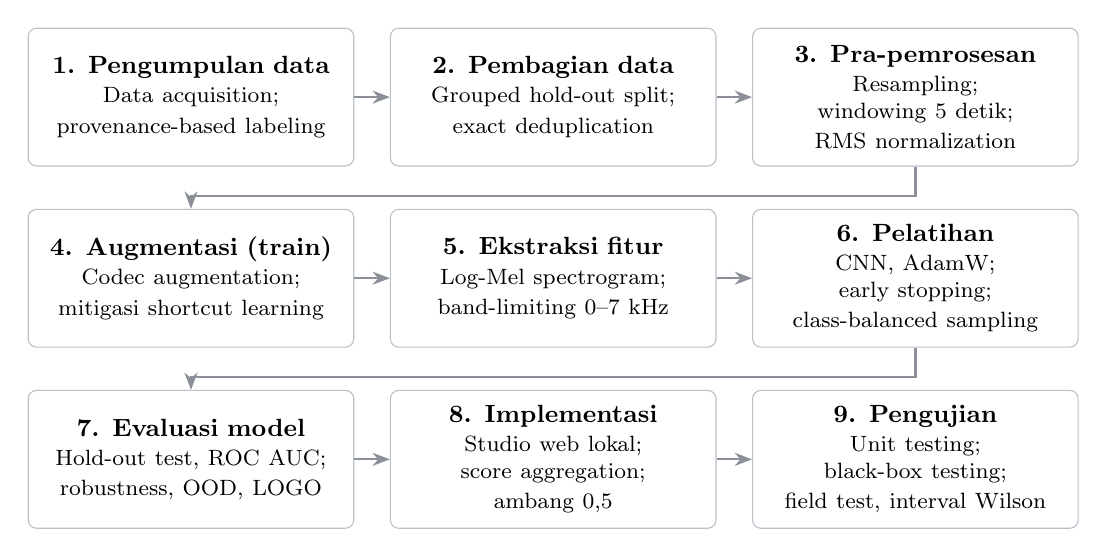
\begin{tikzpicture}[
  tahap/.style={draw=garis, rounded corners=3pt, minimum height=1.75cm, align=center, text width=3.9cm, font=\small},
  panah/.style={-{Stealth[length=2.2mm]}, draw=abu, thick}]
\node[tahap] (s1) at (0,0)    {\textbf{1. Pengumpulan data}\\[1pt]{\footnotesize Data acquisition;\\provenance-based labeling}};
\node[tahap] (s2) at (4.6,0)  {\textbf{2. Pembagian data}\\[1pt]{\footnotesize Grouped hold-out split;\\exact deduplication}};
\node[tahap] (s3) at (9.2,0)  {\textbf{3. Pra-pemrosesan}\\[1pt]{\footnotesize Resampling;\\windowing 5 detik;\\RMS normalization}};
\node[tahap] (s4) at (0,-2.3)   {\textbf{4. Augmentasi (train)}\\[1pt]{\footnotesize Codec augmentation;\\mitigasi shortcut learning}};
\node[tahap] (s5) at (4.6,-2.3) {\textbf{5. Ekstraksi fitur}\\[1pt]{\footnotesize Log-Mel spectrogram;\\band-limiting 0--7 kHz}};
\node[tahap] (s6) at (9.2,-2.3) {\textbf{6. Pelatihan}\\[1pt]{\footnotesize CNN, AdamW;\\early stopping;\\class-balanced sampling}};
\node[tahap] (s7) at (0,-4.6)   {\textbf{7. Evaluasi model}\\[1pt]{\footnotesize Hold-out test, ROC AUC;\\robustness, OOD, LOGO}};
\node[tahap] (s8) at (4.6,-4.6) {\textbf{8. Implementasi}\\[1pt]{\footnotesize Studio web lokal;\\score aggregation;\\ambang 0,5}};
\node[tahap] (s9) at (9.2,-4.6) {\textbf{9. Pengujian}\\[1pt]{\footnotesize Unit testing;\\black-box testing;\\field test, interval Wilson}};
\draw[panah] (s1) -- (s2); \draw[panah] (s2) -- (s3);
\draw[panah] (s3.south) -- ++(0,-0.37) -| (s4.north);
\draw[panah] (s4) -- (s5); \draw[panah] (s5) -- (s6);
\draw[panah] (s6.south) -- ++(0,-0.37) -| (s7.north);
\draw[panah] (s7) -- (s8); \draw[panah] (s8) -- (s9);
\end{tikzpicture}
\caption{Sembilan tahap penelitian.}
\label{fig:peta-metode}
\end{figure}

{\singlespacing\small
\begin{longtable}{L{3.1cm} L{7.0cm} L{2.0cm}}
\caption{Tahap penelitian, nama metode, dan bagian rinciannya.}\label{tab:peta-metode}\\
\toprule
Tahap & Nama metode & Rincian\\
\midrule
\endfirsthead
\toprule
Tahap & Nama metode & Rincian\\
\midrule
\endhead
\bottomrule
\endfoot
1. Pengumpulan data & Data acquisition; provenance-based labeling; random sampling dengan seed & Subbab~\ref{sec:data}\\
2. Pembagian data & Grouped hold-out split (train : validation : test); exact deduplication SHA-256 & Subbab~\ref{sec:split}\\
3. Pra-pemrosesan & Downmixing ke mono; resampling 16 kHz; fixed-length windowing 5 detik; RMS loudness normalization & Subbab~\ref{sec:prapemrosesan}\\
4. Augmentasi (hanya train) & Data augmentation berupa codec augmentation, untuk mitigasi shortcut learning & Subbab~\ref{sec:perbaikan}\\
5. Ekstraksi fitur & Log-Mel spectrogram (STFT + Mel filterbank); band-limiting 0--7 kHz & Subbab~\ref{sec:prapemrosesan}\\
6. Pelatihan & Supervised learning dengan CNN; mini-batch gradient descent (AdamW); class-balanced sampling; mixed precision; early stopping; model checkpointing & Subbab~\ref{sec:pelatihan}\\
7. Evaluasi model & Hold-out test evaluation; disaggregated evaluation; robustness testing; OOD evaluation; leave-one-generator-out; comparative evaluation terhadap baseline & Subbab~\ref{sec:rancangan-evaluasi}\\
8. Implementasi & Aplikasi web lokal; score aggregation (mean pooling); fixed decision threshold & Bab~\ref{bab:panduan}\\
9. Pengujian aplikasi dan lapangan & Unit testing; black-box testing; field test dengan human-in-the-loop feedback; Wilson score interval & Subbab~\ref{sec:rancangan-pengujian}\\
\end{longtable}}

Urutan sebenarnya di kode untuk lagu train adalah: audio didekode, diberi augmentasi codec, dijadikan mono 16 kHz, dipotong per 5 detik, dinormalisasi RMS, lalu diubah menjadi spektrogram log-Mel. Tahap 3 dan 4 dipisah pada peta di atas supaya mudah dijelaskan.

\section{Data}\label{sec:data}
Data latih dikumpulkan dari tiga sumber (Tabel~\ref{tab:sumber-data}). Label manusia atau AI ditentukan dari asal-usul data (\textit{provenance-based labeling}), bukan dari tebakan pendengaran. Subset MUSEBENCH dipilih acak dengan seed 42 sehingga pemilihannya dapat diulang.

\begin{table}[htbp]
\centering
\singlespacing\small
\caption{Sumber data latih.}
\label{tab:sumber-data}
\begin{tabularx}{\textwidth}{Y L{1.6cm} L{2.4cm} L{3.4cm}}
\toprule
Sumber & Kelas & Jumlah lagu & Format\\
\midrule
SONICS (Suno chirp v2/v3/v3.5, Udio) \cite{rahman2025sonics} & AI & 20.000 & MP3 kualitas rendah\\
FMA-small \cite{defferrard2017fma} & Manusia & 7.997 & MP3 $\pm$300 kbps, 44,1 kHz\\
MUSEBENCH Jamendo dan OOD FMA \cite{musebench} & Manusia & 3.689 & MP3\\
MUSEBENCH: MusicGen, AudioLDM, Riffusion, JASCO, Magenta, Stable Audio \cite{musebench} & AI & 4.080 (680 per generator) & WAV 32 kHz\\
\bottomrule
\end{tabularx}
\end{table}

Tautan unduhan setiap dataset tercantum pada Lampiran~D.

\section{Pembagian Data}\label{sec:split}
Data dibagi dengan \textit{hold-out validation} tiga bagian (\textit{train}--\textit{validation}--\textit{test split}) yang dilakukan per kelompok lagu (\textit{grouped hold-out split}). Lagu Jamendo dan semua versi AI yang dibuat dari lagu itu berada di satu kelompok, dan satu kelompok tidak pernah terbelah ke dua bagian. Cara ini mencegah \textit{data leakage}. File yang byte-identik dari dua sumber hanya disimpan sekali (\textit{exact deduplication} dengan hash SHA-256).

\begin{table}[htbp]
\centering
\singlespacing\small
\caption{Rasio pembagian data per sumber.}
\label{tab:rasio}
\begin{tabularx}{\textwidth}{L{3.6cm} L{3.4cm} Y}
\toprule
Sumber data & Train : validation : test & Cara pembagian\\
\midrule
SONICS + FMA-small & 82,4 : 7,6 : 10,0 & \textit{Predefined split}, mengikuti pembagian resmi dataset SONICS\\
MUSEBENCH & 70 : 15 : 15 & \textit{Grouped random split} berbasis hash SHA-256 dari \kode{group\_id} dan seed 42\\
Gabungan (data final) & 79,9 : 9,1 : 10,9 & 28.587 : 3.268 : 3.911 lagu\\
\bottomrule
\end{tabularx}
\end{table}

\textit{K-fold cross-validation} tidak dipakai karena melatih model berkali-kali dengan $\pm$36.000 lagu dan $\pm$500.000 segmen train terlalu mahal untuk kuota GPU Google Colab. Dengan data sebanyak ini, satu \textit{hold-out test} berisi 3.911 lagu sudah memberi estimasi yang stabil. Generalisasi ke generator baru diuji dengan \textit{leave-one-generator-out} (Subbab~\ref{sec:rancangan-evaluasi}).

\section{Pra-pemrosesan dan Ekstraksi Fitur}\label{sec:prapemrosesan}
Setiap rekaman dipotong menjadi segmen 5 detik, setiap segmen diubah menjadi spektrogram log-Mel, CNN memberi skor AI per segmen, lalu skor dirata-ratakan menjadi satu vonis (Gambar~\ref{fig:alur}).

\begin{figure}[htbp]
\centering
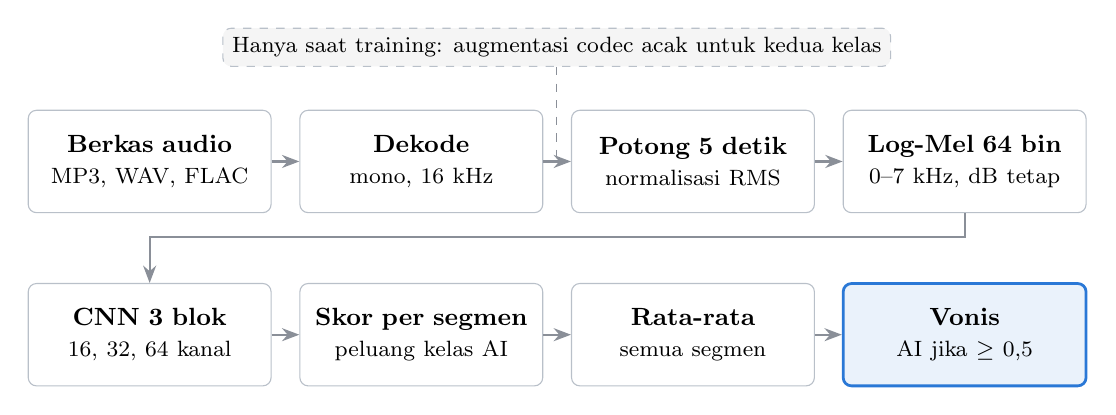
\begin{tikzpicture}[
  kotak/.style={draw=garis, rounded corners=3pt, minimum height=1.3cm, align=center, text width=2.85cm, font=\small},
  panah/.style={-{Stealth[length=2.2mm]}, draw=abu, thick}]
\node[kotak] (a1) at (0,0)    {\textbf{Berkas audio}\\{\footnotesize MP3, WAV, FLAC}};
\node[kotak] (a2) at (3.45,0) {\textbf{Dekode}\\{\footnotesize mono, 16 kHz}};
\node[kotak] (a3) at (6.9,0)  {\textbf{Potong 5 detik}\\{\footnotesize normalisasi RMS}};
\node[kotak] (a4) at (10.35,0){\textbf{Log-Mel 64 bin}\\{\footnotesize 0--7 kHz, dB tetap}};
\node[kotak] (b1) at (0,-2.2)    {\textbf{CNN 3 blok}\\{\footnotesize 16, 32, 64 kanal}};
\node[kotak] (b2) at (3.45,-2.2) {\textbf{Skor per segmen}\\{\footnotesize peluang kelas AI}};
\node[kotak] (b3) at (6.9,-2.2)  {\textbf{Rata-rata}\\{\footnotesize semua segmen}};
\node[kotak, draw=aksen, fill=aksen!10, line width=1pt] (b4) at (10.35,-2.2) {\textbf{Vonis}\\{\footnotesize AI jika $\ge$ 0,5}};
\node[draw=garis, dashed, rounded corners=3pt, fill=black!4, font=\footnotesize, align=center] (catatan) at (5.17,1.45) {Hanya saat training: augmentasi codec acak untuk kedua kelas};
\draw[panah] (a1) -- (a2); \draw[panah] (a2) -- (a3); \draw[panah] (a3) -- (a4);
\draw[panah] (a4.south) -- ++(0,-0.3) -| (b1.north);
\draw[panah] (b1) -- (b2); \draw[panah] (b2) -- (b3); \draw[panah] (b3) -- (b4);
\draw[abu, dashed] (catatan.south) -- (5.17,0);
\end{tikzpicture}
\caption{Alur analisis dari berkas audio sampai vonis.}
\label{fig:alur}
\end{figure}

Rinciannya sama untuk pelatihan dan analisis di studio:
\begin{itemize}
\item audio didekode, dijadikan mono (\textit{downmixing}), dan di-\textit{resample} ke 16 kHz;
\item rekaman dibaca per jendela 5 detik tanpa tumpang tindih (\textit{fixed-length windowing}); potongan terakhir yang pendek diisi nol;
\item RMS setiap jendela disetel ke $-20$ dBFS (\textit{loudness normalization}), sehingga keras-pelannya rekaman tidak menjadi petunjuk;
\item spektrogram log-Mel 64 pita, FFT 1024, \textit{hop} 256, rentang 0--7 kHz, skala dB tetap ($-80$ sampai $+20$ dB) tanpa normalisasi berbasis dataset.
\end{itemize}

\section{Perbaikan terhadap Shortcut Learning}\label{sec:perbaikan}
Data latih menyimpan beberapa perbedaan teknis antara kelas AI dan manusia yang dapat dijadikan jalan pintas oleh model. Tabel~\ref{tab:perbaikan} merangkum perbedaan tersebut, cara mencegahnya, dan opsi perintah yang mengaktifkannya.

{\singlespacing\small
\begin{longtable}{L{3.1cm} L{6.3cm} L{2.9cm}}
\caption{Potensi jalan pintas pada data dan cara mencegahnya.}\label{tab:perbaikan}\\
\toprule
Potensi jalan pintas & Pencegahan & Opsi perintah\\
\midrule
\endfirsthead
\toprule
Potensi jalan pintas & Pencegahan & Opsi perintah\\
\midrule
\endhead
\bottomrule
\endfoot
Codec dan bitrate berbeda per kelas & Setiap lagu train (kedua kelas) dibuat 3 versi dengan rantai acak: MP3/AAC/Opus/PCM 32--320 kbps, \textit{resample} 16--48 kHz, mono/stereo, gain $-12$ sampai $+4$ dB, lowpass acak 4--7,9 kHz & \kode{--augment-variants 3}\\
Pita di atas 7,3 kHz hanya ada pada lagu manusia & Spektrogram dibatasi 0--7 kHz (\textit{band-limiting}), sebab augmentasi tidak dapat menambah bandwidth ke lagu AI & \kode{--fmax 7000}\\
Keras-pelan rekaman & Normalisasi RMS per jendela & \kode{--loudness-norm}\\
Kelas tidak seimbang & \textit{Weighted random sampling}: setiap kelas, dan setiap generator di dalamnya, mendapat porsi sampel sama & \kode{--balance sampler --balance-by generator}\\
Hanya dua generator AI & Data tambahan MUSEBENCH: Jamendo, OOD FMA, dan enam generator lain & \kode{hmf.manifest musebench}\\
\end{longtable}}

Rantai augmentasi ditentukan oleh seed, hash SHA-256 file, dan nomor varian, sehingga hasilnya dapat diulang. Data validation dan test tidak diaugmentasi agar evaluasinya bersih.

\section{Model dan Pelatihan}\label{sec:pelatihan}
Model adalah CNN tiga blok konvolusi (16, 32, dan 64 kanal), masing-masing konvolusi $3\times3$, ReLU, dan \textit{max-pooling} $2\times2$. Varian \kode{frequency} mempertahankan 8 posisi frekuensi saat \textit{pooling}, lalu dropout 0,2 dan lapisan linear ke dua kelas. Keluaran softmax kelas AI menjadi skor segmen. Pengaturan pelatihan dirangkum pada Tabel~\ref{tab:hyper}.

\begin{table}[htbp]
\centering
\singlespacing\small
\caption{Pengaturan pelatihan model final.}
\label{tab:hyper}
\begin{tabularx}{\textwidth}{L{4.6cm} Y}
\toprule
Pengaturan & Nilai\\
\midrule
Metode & \textit{Supervised learning}, bobot awal acak, tanpa bobot pralatih\\
Loss & \textit{Cross-entropy}\\
Optimizer & AdamW, \textit{learning rate} 0,001, \textit{weight decay} 0,0001\\
Ukuran batch & 64 segmen\\
Penyeimbangan kelas & \textit{Weighted random sampling} per kelas dan per generator\\
Pemilihan model & Loss validasi terendah (\textit{model checkpointing})\\
Penghentian & \textit{Early stopping}, \textit{patience} 5 epoch, maksimal 30 epoch\\
Percepatan & \textit{Mixed precision} (AMP) di GPU Google Colab\\
Agregasi & Rata-rata skor segmen; ambang keputusan 0,5 ditetapkan sebelum melihat data test\\
\bottomrule
\end{tabularx}
\end{table}

\section{Pelaksanaan di Google Colab}
Notebook \kode{colab/train.ipynb} menjalankan pelatihan penuh di Google Colab. Pekerjaannya dibagi menjadi sesi CPU untuk menyiapkan fitur, yang dapat dicicil lintas sesi, dan sesi GPU untuk pelatihan. Tabel~\ref{tab:colab} memberi nama metode untuk setiap langkah notebook.

{\singlespacing\small
\begin{longtable}{L{0.5cm} L{2.4cm} L{5.0cm} L{3.9cm}}
\caption{Langkah pemrosesan di Google Colab dan nama metodenya.}\label{tab:colab}\\
\toprule
No & Langkah & Yang dilakukan & Nama metode\\
\midrule
\endfirsthead
\toprule
No & Langkah & Yang dilakukan & Nama metode\\
\midrule
\endhead
\bottomrule
\endfoot
1 & Salin audio & Zip SONICS dan FMA disalin ke disk lokal Colab lalu diekstrak & Data acquisition\\
2 & Pilih MUSEBENCH & Subset acak ber-seed, dikecilkan otomatis agar muat di disk; hanya file terpilih yang diunduh & Random sampling dengan seed; partial download (HTTP Range)\\
3 & Beri label & Label dari folder asal data & Provenance-based labeling\\
4 & Bagi data & Train/validation/test per kelompok & Grouped hold-out split\\
5 & Buang duplikat & File dengan hash sama disimpan sekali & Exact deduplication\\
6 & Dekode audio & Stereo jadi mono, resample 16 kHz & Downmixing dan resampling\\
7 & Potong rekaman & Jendela 5 detik, potongan terakhir diisi nol & Fixed-length windowing, zero padding\\
8 & Samakan kerasnya suara & RMS tiap jendela $-20$ dBFS & RMS loudness normalization\\
9 & Augmentasi (train) & 3 versi codec acak per lagu untuk kedua kelas; diterapkan sebelum langkah 6--8 & Codec augmentation\\
10 & Ekstraksi fitur & STFT 1024/hop 256, 64 filter Mel, dibatasi 0--7 kHz & Log-Mel spectrogram; band-limiting\\
11 & Simpan cache & Fitur float16 per 100 lagu ke Google Drive, dapat dilanjutkan & Feature caching; checkpointed batch processing\\
12 & Pelatihan & CNN, cross-entropy, AdamW, batch 64 & Mini-batch gradient descent\\
13 & Seimbangkan kelas & Porsi sampel sama per kelas dan generator & Class-balanced sampling\\
14 & Percepat di GPU & Perhitungan float16 otomatis & Mixed precision training\\
15 & Pilih model & Simpan bobot terbaik; berhenti setelah 5 epoch tanpa perbaikan; dapat dilanjutkan & Model checkpointing; early stopping; resume training\\
16 & Vonis satu lagu & Rata-rata skor segmen dibanding ambang 0,5 & Score aggregation; fixed decision threshold\\
\end{longtable}}

\section{Rancangan Evaluasi}\label{sec:rancangan-evaluasi}
Model dievaluasi dengan tujuh langkah (Tabel~\ref{tab:evaluasi}) memakai metrik pada Persamaan~\eqref{eq:acc}--\eqref{eq:wilson}. Untuk uji \textit{robustness} dipakai dua metrik tambahan: \textit{mean} $|\Delta|$, yaitu rata-rata perubahan skor setelah lagu dikompres ulang, dan \textit{flip rate}, yaitu persentase lagu yang vonisnya berbalik. Model yang baik memiliki keduanya mendekati nol.

{\singlespacing\small
\begin{longtable}{L{0.5cm} L{2.6cm} L{4.4cm} L{4.3cm}}
\caption{Langkah uji coba model dan nama metodenya.}\label{tab:evaluasi}\\
\toprule
No & Langkah uji & Pertanyaan yang dijawab & Nama metode\\
\midrule
\endfirsthead
\toprule
No & Langkah uji & Pertanyaan yang dijawab & Nama metode\\
\midrule
\endhead
\bottomrule
\endfoot
1 & Uji pada data test & Seberapa akurat model pada data yang belum pernah dipakai? & Hold-out test evaluation\\
2 & Rincian per generator & Generator mana yang sulit dideteksi? & Disaggregated evaluation\\
3 & Kompres ulang lagu test & Apakah vonis berubah hanya karena format file? & Robustness testing (MP3 32k, MP3 128k, AAC 128k, Opus 64k)\\
4 & Lagu dari luar dataset & Apakah model berguna untuk lagu dari sumber lain? & Out-of-distribution evaluation\\
5 & Generator ditahan dari training & Apakah model mengenali generator yang belum pernah dilihat? & Leave-one-generator-out\\
6 & Matikan perbaikan satu per satu & Komponen mana yang paling berpengaruh? & Ablation study\\
7 & Umpan balik pengguna & Seberapa sering model benar pada lagu sungguhan? & Field test; Wilson score interval\\
\end{longtable}}

\section{Rancangan Pengujian Perangkat Lunak}\label{sec:rancangan-pengujian}
Aplikasi diuji dengan dua metode. \textit{Unit testing} dan \textit{integration testing} memakai pytest: 42 tes otomatis memeriksa antara lain augmentasi yang deterministik dan berlaku untuk kedua kelas, data validation/test yang tidak diaugmentasi, \textit{balanced sampler}, pembagian per kelompok tanpa kebocoran, deduplikasi, pemrosesan yang dicicil, lanjutan pelatihan, umpan balik, dan endpoint server. \textit{Black-box testing} menguji studio web hanya dari masukan dan keluarannya tanpa melihat kode \cite{myers2011art}; skenario dan hasilnya disajikan pada Subbab~\ref{sec:hasil-blackbox}.

\chapter{PANDUAN PENGGUNAAN}\label{bab:panduan}

\section{Kebutuhan Sistem}
Studio web cukup dijalankan di laptop Windows biasa; GPU hanya dibutuhkan untuk melatih ulang model dengan data penuh (Tabel~\ref{tab:kebutuhan}). FFmpeg tidak perlu dipasang terpisah karena paket \kode{imageio-ffmpeg} membawa program ffmpeg sendiri.

\begin{table}[htbp]
\centering
\singlespacing\small
\caption{Kebutuhan sistem.}
\label{tab:kebutuhan}
\begin{tabularx}{\textwidth}{L{2.6cm} L{4.6cm} Y}
\toprule
Komponen & Kebutuhan & Catatan\\
\midrule
Sistem operasi & Windows 10/11 64-bit & Kode juga berjalan di Linux (dipakai di Google Colab)\\
Python & 3.11 atau lebih baru, 64-bit & Diuji dengan Python 3.14\\
RAM & 8 GB & 16 GB disarankan untuk pelatihan lokal\\
Disk & $\pm$1 GB untuk kode dan environment & Dataset dan cache fitur membutuhkan puluhan GB\\
GPU & Opsional & Pelatihan penuh dijalankan di Google Colab\\
Paket Python & torch, numpy, librosa, soundfile, scikit-learn, pytest, imageio-ffmpeg & Tercantum di \kode{requirements.txt}\\
\bottomrule
\end{tabularx}
\end{table}

\section{Instalasi}\label{sec:instalasi}
Jalankan perintah berikut di PowerShell dari folder proyek hasil \kode{git clone}:
\begin{enumerate}
\item Buat environment Python dan perbarui pip:
\begin{Perintah}
py -3.14 -m venv .venv
.\.venv\Scripts\python.exe -m pip install --upgrade pip
\end{Perintah}
\item Pasang PyTorch sesuai petunjuk di \url{https://pytorch.org/get-started/locally/}; versi CPU cukup untuk studio web.
\item Pasang paket lainnya:
\begin{Perintah}
.\.venv\Scripts\python.exe -m pip install -r requirements.txt
\end{Perintah}
\item Jalankan tes otomatis. Hasil yang diharapkan: 42 tes lulus.
\begin{Perintah}
.\.venv\Scripts\python.exe -m pytest -q
\end{Perintah}
\end{enumerate}
Simpan daftar versi paket dengan \kode{pip freeze > environment-lock.txt} setiap kali menjalankan eksperimen agar hasilnya dapat diulang.

Model final sudah disertakan di repositori pada folder \kode{runs/hmf-aug-v2/}, sehingga studio dapat langsung dipakai setelah instalasi tanpa melatih ulang. Hanya file yang diperlukan yang disimpan (Tabel~\ref{tab:file-model}); file indeks cache berukuran $\pm$282 MB dan \kode{last.pt} tidak disertakan karena hanya dipakai saat pelatihan dan bisa dibuat ulang.

\begin{table}[htbp]
\centering
\singlespacing\small
\caption{File model final di repositori.}
\label{tab:file-model}
\begin{tabularx}{\textwidth}{L{5.1cm} L{1.4cm} Y}
\toprule
File & Ukuran & Kegunaan\\
\midrule
\kode{best.pt} & 0,1 MB & Bobot CNN terbaik (epoch 27); wajib untuk analisis\\
\kode{report.json} & 0,9 MB & Konfigurasi audio, arsitektur, dan metrik test; wajib untuk analisis dan panel model\\
\kode{history.json} & 0,04 MB & Loss dan metrik per epoch\\
\kode{cache\_audio\_config.json},\newline \kode{cache\_prepare\_config.json} & $<$0,01 MB & Pengaturan ekstraksi fitur saat pelatihan\\
\kode{cache\_skipped.json} & $<$0,01 MB & Daftar lagu yang gagal didekode saat pra-pemrosesan\\
\kode{manifest-musebench.csv} & 1,1 MB & Daftar lagu MUSEBENCH yang dipakai\\
\bottomrule
\end{tabularx}
\end{table}

\section{Menjalankan Studio Web}
Studio web dibuka dengan satu perintah, lalu dipakai lewat browser di alamat \url{http://127.0.0.1:8765}. Server hanya menerima koneksi dari komputer yang sama.
\begin{enumerate}
\item Buka PowerShell di folder proyek, lalu jalankan studio. Tanpa opsi, server memakai model terbaru di folder \kode{runs/}; opsi \kode{--run} memilih model tertentu.
\begin{Perintah}
.\.venv\Scripts\python.exe -m hmf.web --run runs/hmf-aug-v2
\end{Perintah}
\item Terminal menampilkan nama model aktif dan alamat studio. Buka alamat itu di browser (Gambar~\ref{fig:halaman-awal}).
\item Tarik file audio ke kotak unggah atau klik kotak itu untuk memilih file. Nama file dan pemutar audio akan tampil (Gambar~\ref{fig:file-dipilih}).
\item Klik \textbf{Analisis rekaman}. Lagu 3 menit biasanya selesai dalam beberapa detik di CPU.
\item Hentikan server dengan Ctrl+C di terminal.
\end{enumerate}
Pojok kanan atas halaman selalu menampilkan nama model yang aktif. Jika port 8765 sudah dipakai, misalnya karena studio lain masih berjalan, server menolak berjalan dan menyarankan memakai \kode{--port} lain.

\begin{figure}[htbp]
\centering
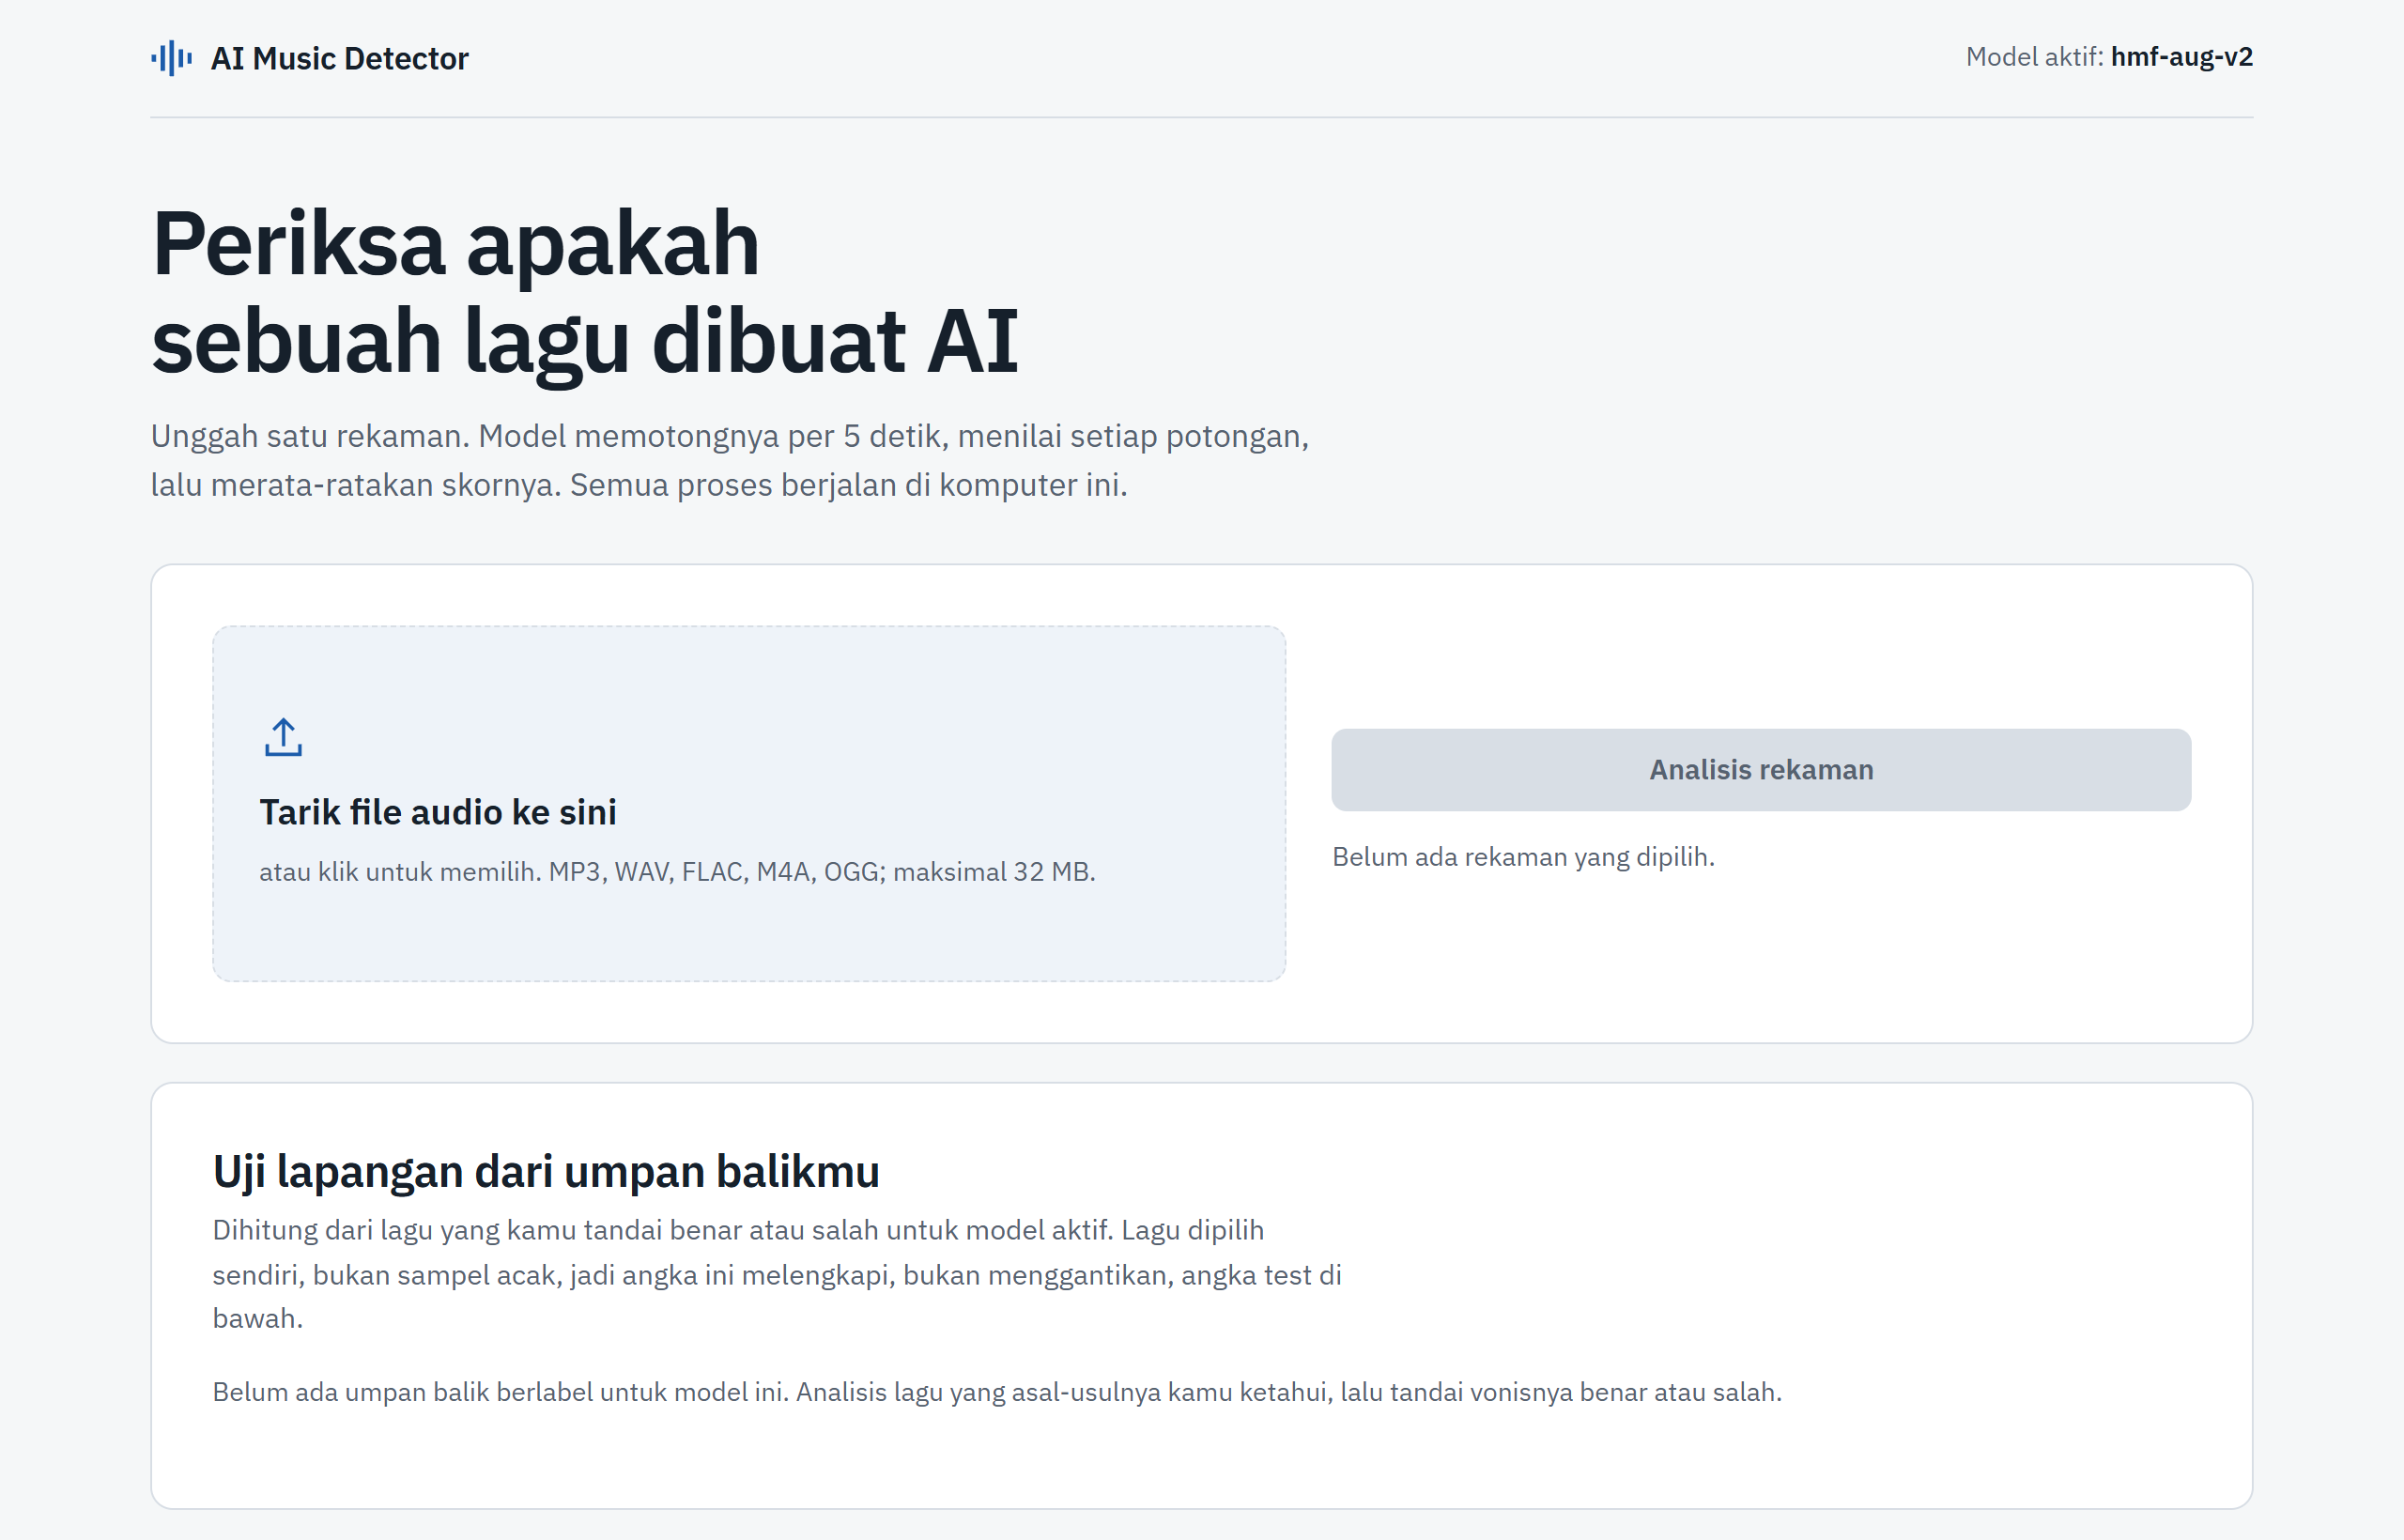
\includegraphics[width=0.95\textwidth]{01-halaman-awal.png}
\caption{Halaman awal studio dengan kotak unggah dan nama model aktif.}
\label{fig:halaman-awal}
\end{figure}

\begin{figure}[htbp]
\centering
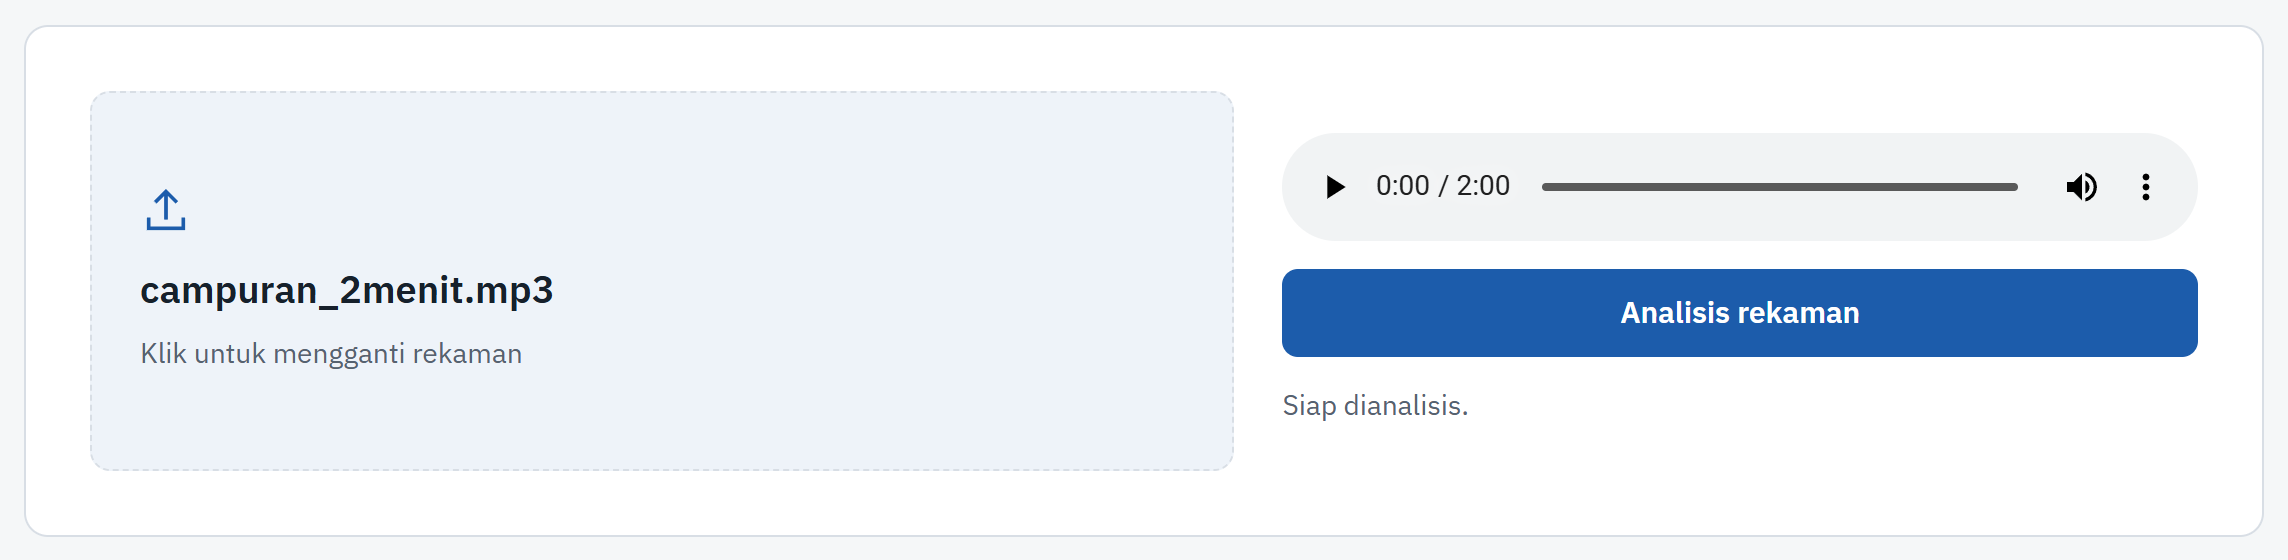
\includegraphics[width=0.95\textwidth]{02-file-dipilih.png}
\caption{Kotak unggah setelah file dipilih.}
\label{fig:file-dipilih}
\end{figure}

\section{Membaca Hasil Analisis}
Vonis ditentukan oleh satu angka: rata-rata skor AI semua segmen 5 detik. Jika rata-rata itu mencapai ambang 50\%, vonisnya AI; jika di bawahnya, Human. Tabel~\ref{tab:bagian-layar} menjelaskan setiap bagian layar hasil. Gambar pada subbab ini menunjukkan tata letak tampilan; angka di dalamnya berbeda untuk setiap lagu.

{\singlespacing\small
\begin{longtable}{L{2.6cm} L{4.6cm} L{5.1cm}}
\caption{Bagian layar hasil analisis.}\label{tab:bagian-layar}\\
\toprule
Bagian layar & Isi & Cara membacanya\\
\midrule
\endfirsthead
\toprule
Bagian layar & Isi & Cara membacanya\\
\midrule
\endhead
\bottomrule
\endfoot
Vonis & Kata \textbf{AI} (oranye) atau \textbf{Human} (biru) & Hasil akhir model untuk seluruh rekaman\\
Skor AI & Persentase, misalnya 51,46\% & Rata-rata skor segmen; makin dekat 100\% makin mirip data AI\\
\kode{ai\_score} & Angka mentah, misalnya 0.5146298917631308 & Nilai yang sama persis dengan di JSON\\
Meter & Batang 0--100\% dengan garis di ambang & Jarak ujung batang ke garis menunjukkan seberapa yakin vonisnya\\
Spektrogram & Energi per frekuensi (0--7 kHz) terhadap waktu & Persis masukan yang dilihat CNN\\
Skor per segmen & Satu batang per 5 detik, oranye jika $\ge$ ambang & Menunjukkan bagian lagu yang mendorong vonis\\
Pilih segmen & Penggeser dan teks keterangan & Pemutar audio melompat ke awal segmen yang dipilih\\
Data JSON & Laporan lengkap & Dapat dilihat atau diunduh untuk dokumentasi\\
\end{longtable}}

Persentase dibulatkan dua desimal tanpa melewati ambang atau batas: skor 0,49996 tampil 49,99\% (bukan 50,00\%), skor sangat kecil tampil $<$0,01\%, dan skor hampir 1 tampil $>$99,99\%. Spektrogram dan batang skor memakai sumbu waktu yang sama. Arahkan kursor ke batang untuk melihat nomor segmen, rentang waktu, dan skornya, lalu klik untuk memilih segmen.

Gambar~\ref{fig:vonis} dan~\ref{fig:spektrogram} memperlihatkan hasil untuk rekaman campuran 2 menit. Enam segmen pertama (lagu FMA) berada di bawah ambang, sedangkan sebagian besar segmen berikutnya (lagu Udio dan Suno) di atas ambang. Rata-ratanya 51,46\%, sehingga vonisnya AI dengan selisih tipis. Vonis setipis ini sebaiknya dibaca bersama grafik segmen, bukan sebagai kepastian.

\begin{figure}[htbp]
\centering
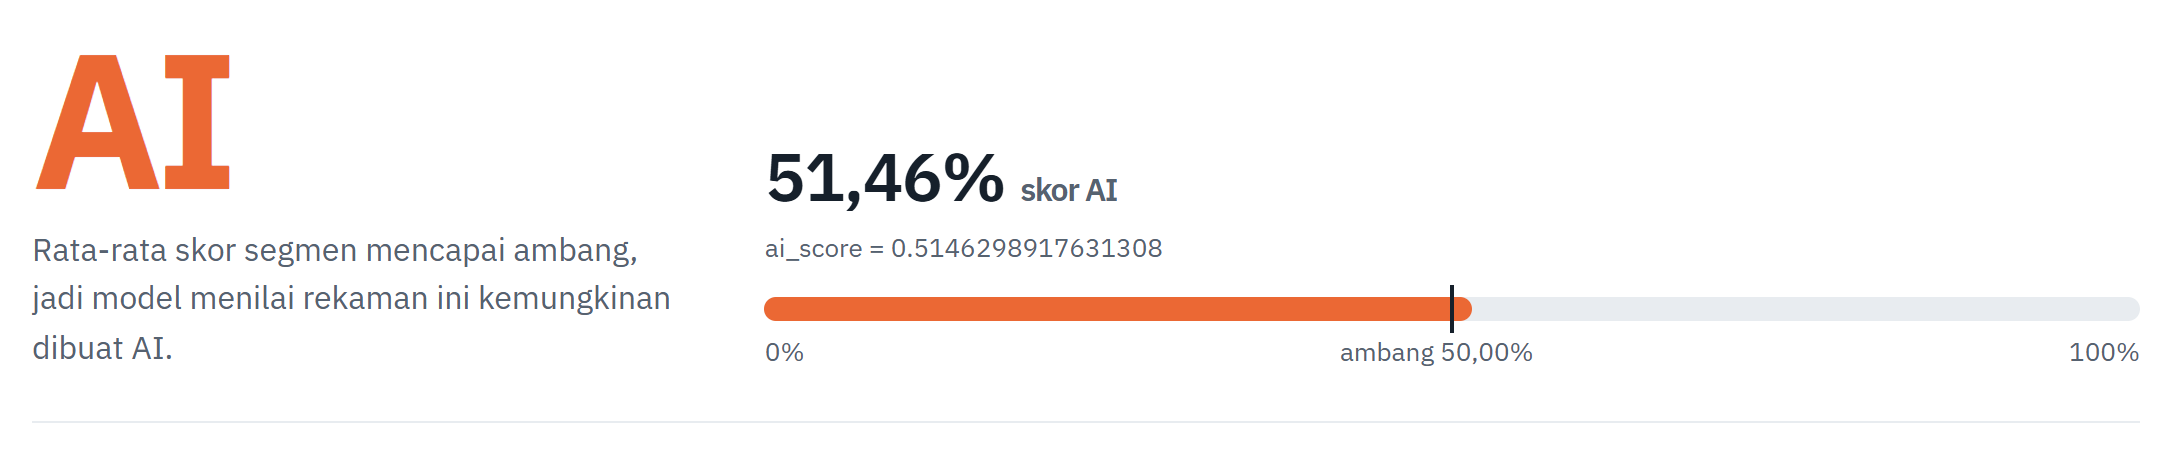
\includegraphics[width=0.95\textwidth]{03-hasil-vonis.png}
\caption{Vonis, skor AI, nilai \kode{ai\_score}, dan meter terhadap ambang.}
\label{fig:vonis}
\end{figure}

\begin{figure}[htbp]
\centering
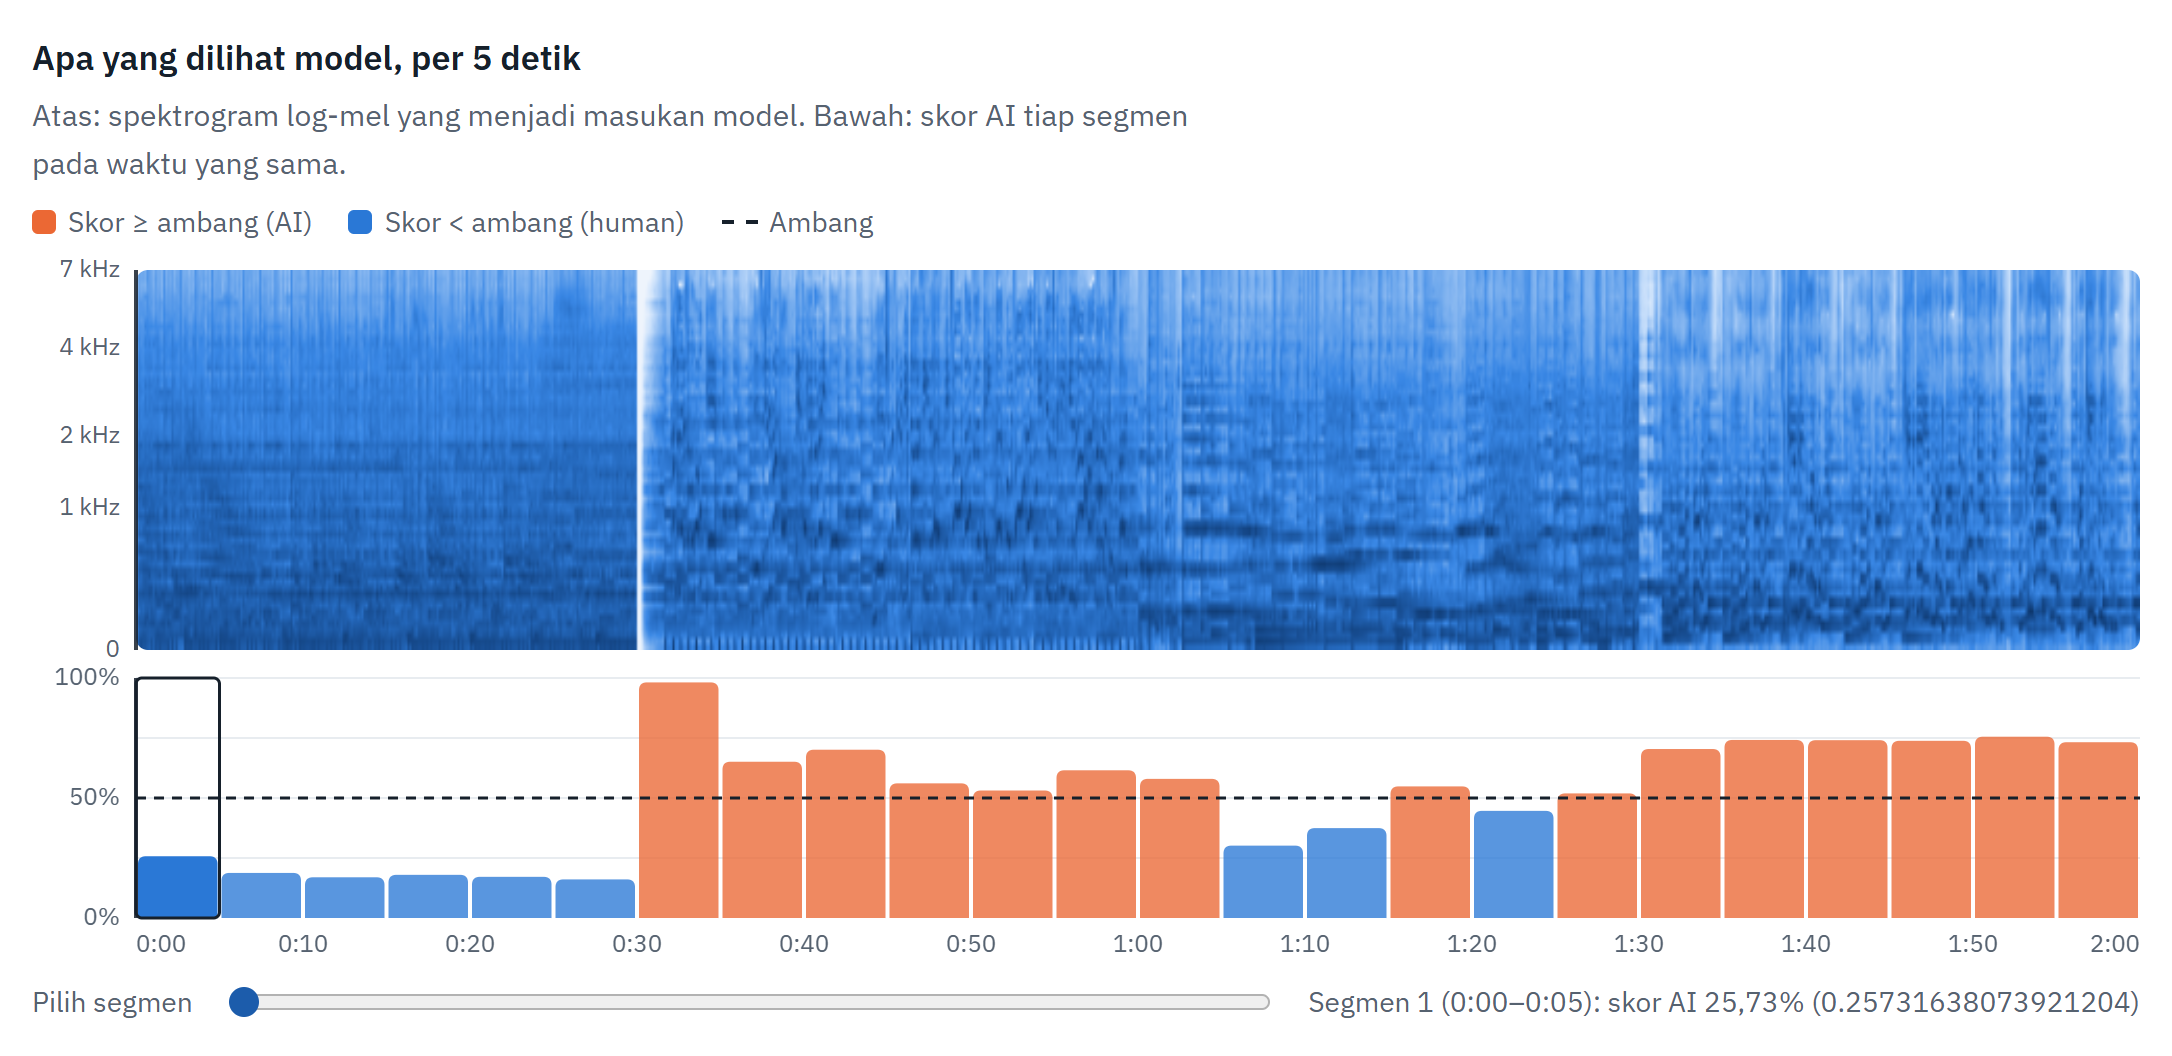
\includegraphics[width=0.95\textwidth]{04-spektrogram-skor.png}
\caption{Spektrogram log-Mel dan skor AI per segmen 5 detik pada sumbu waktu yang sama.}
\label{fig:spektrogram}
\end{figure}

\begin{figure}[htbp]
\centering
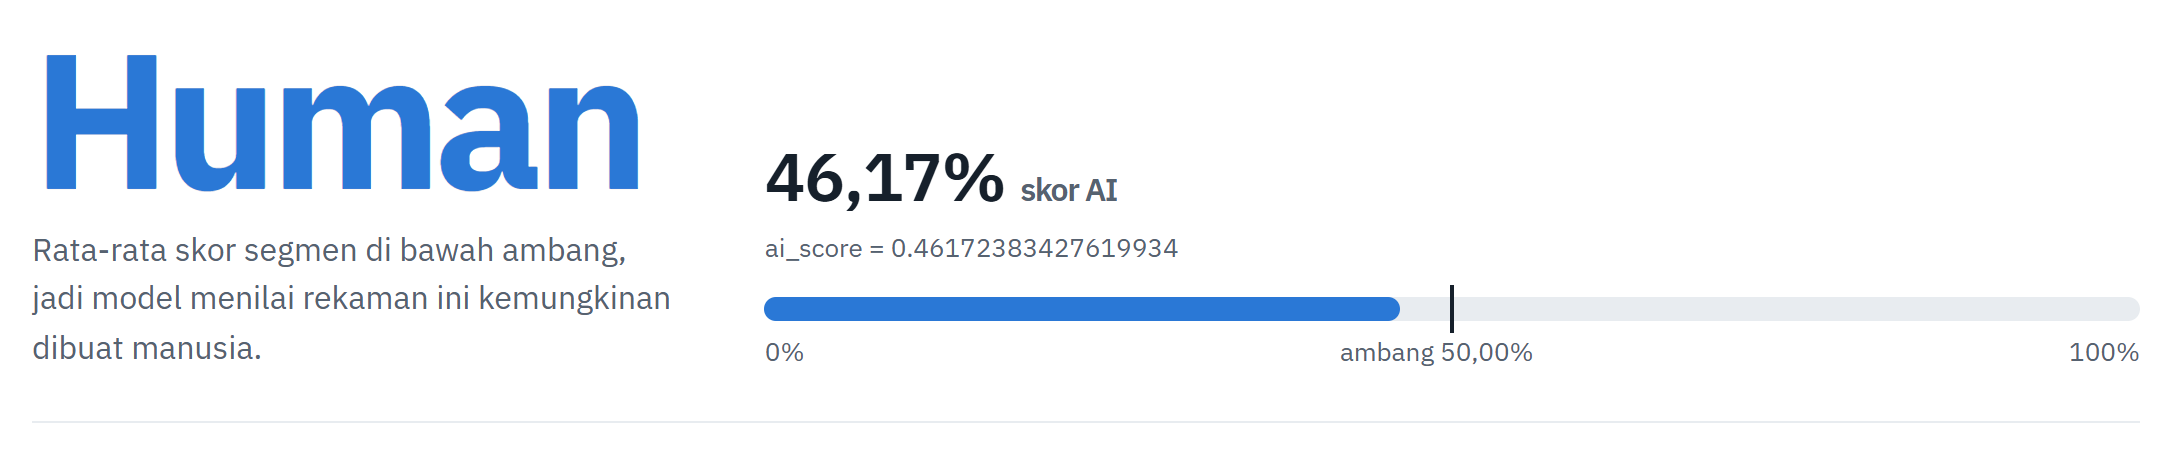
\includegraphics[width=0.95\textwidth]{08-contoh-human.png}
\caption{Contoh vonis Human untuk lagu FMA dengan skor 46,17\%.}
\label{fig:contoh-human}
\end{figure}

Studio juga dapat dibuka di layar ponsel; semua bagian tersusun dalam satu kolom (Gambar~\ref{fig:ponsel}). Laporan JSON berisi \kode{status}, \kode{filename}, \kode{result} (vonis, skor, ambang, cara agregasi, panjang dan jumlah segmen, serta skor per segmen), dan \kode{metadata} (arsitektur, nama run, dan waktu proses). Contoh lengkapnya ada pada Lampiran~C.

\begin{figure}[htbp]
\centering
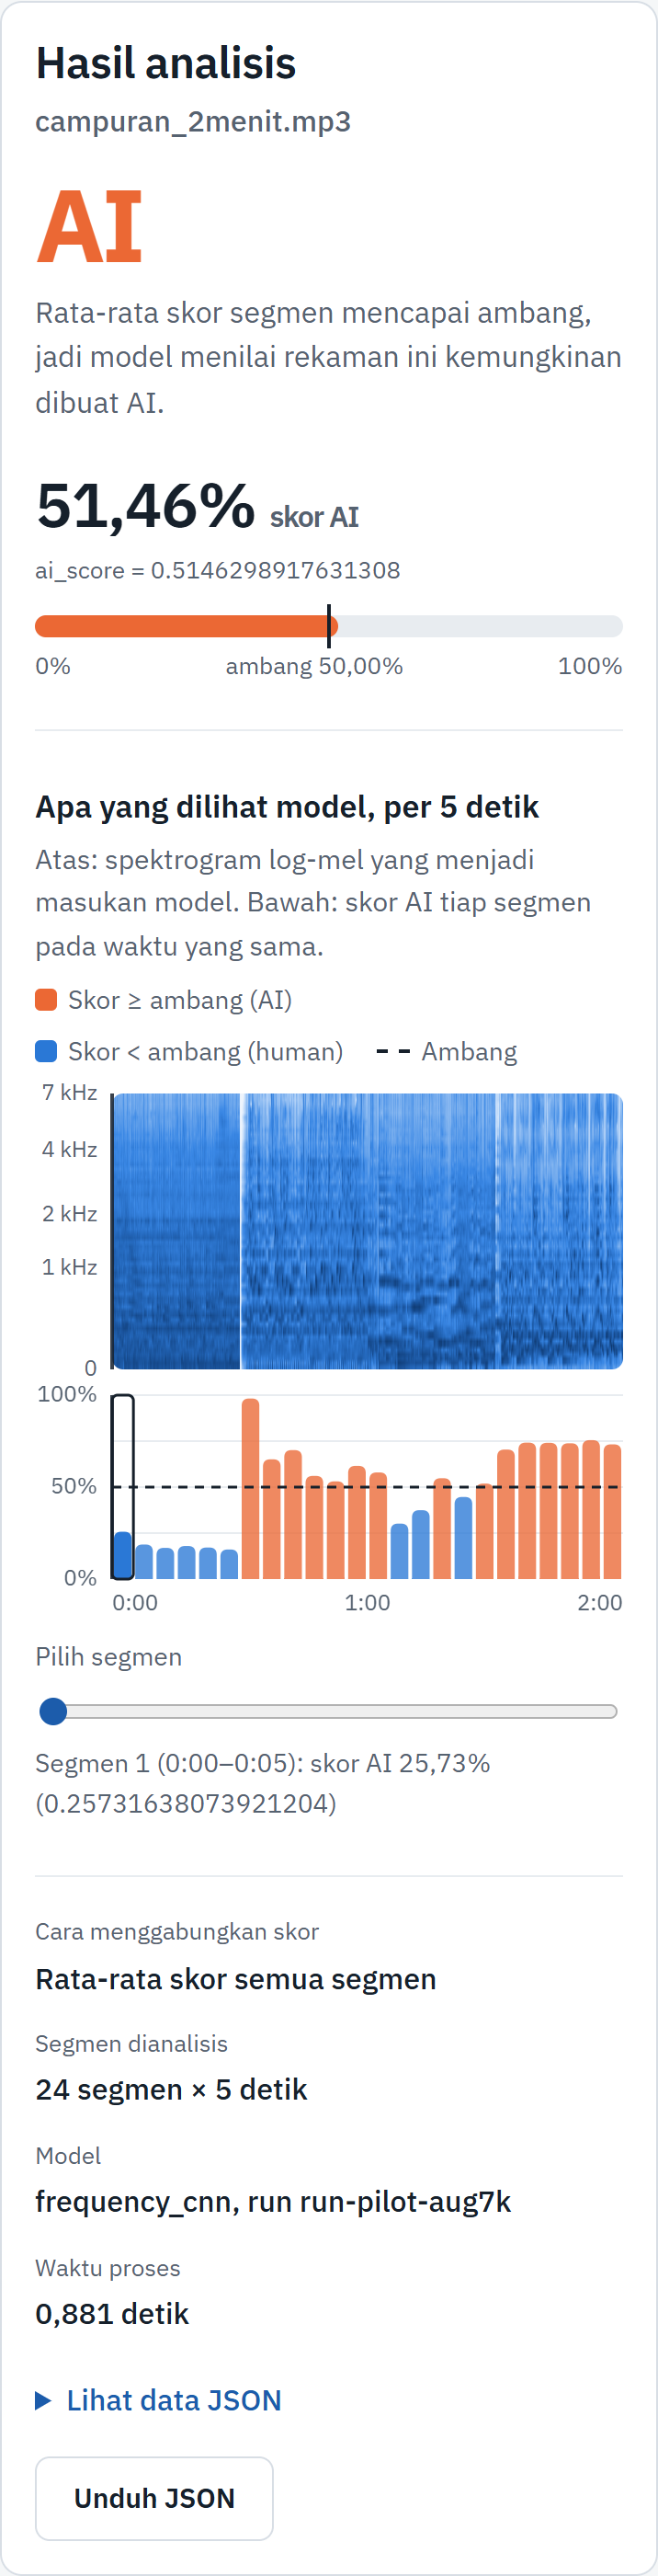
\includegraphics[height=0.62\textheight]{09-tampilan-hp.png}
\caption{Hasil analisis pada layar ponsel dengan lebar 390 piksel.}
\label{fig:ponsel}
\end{figure}

\section{Memberi Umpan Balik}
Setelah vonis muncul, pengguna dapat menandai apakah vonis itu benar. Kumpulan jawaban ini menjadi uji lapangan, yaitu ukuran seberapa sering model benar pada lagu sungguhan yang diperiksa pengguna.
\begin{enumerate}
\item Analisis lagu yang asal-usulnya diketahui.
\item Pada kartu \textbf{Apakah vonis ini benar?}, pilih \textbf{Benar}, \textbf{Salah}, atau \textbf{Tidak tahu}.
\item Untuk Benar atau Salah, pilih sumber label (wajib): dibuat sendiri, label resmi platform, dataset dengan asal-usul jelas, konfirmasi pembuat, atau lainnya.
\item Centang \textbf{Simpan salinan audio} hanya jika berhak menyimpannya dan ingin lagu itu dipakai untuk evaluasi atau pelatihan ulang.
\item Klik \textbf{Simpan umpan balik}. Untuk lagu dan model yang sama, jawaban terakhir yang dipakai.
\end{enumerate}

\begin{figure}[htbp]
\centering
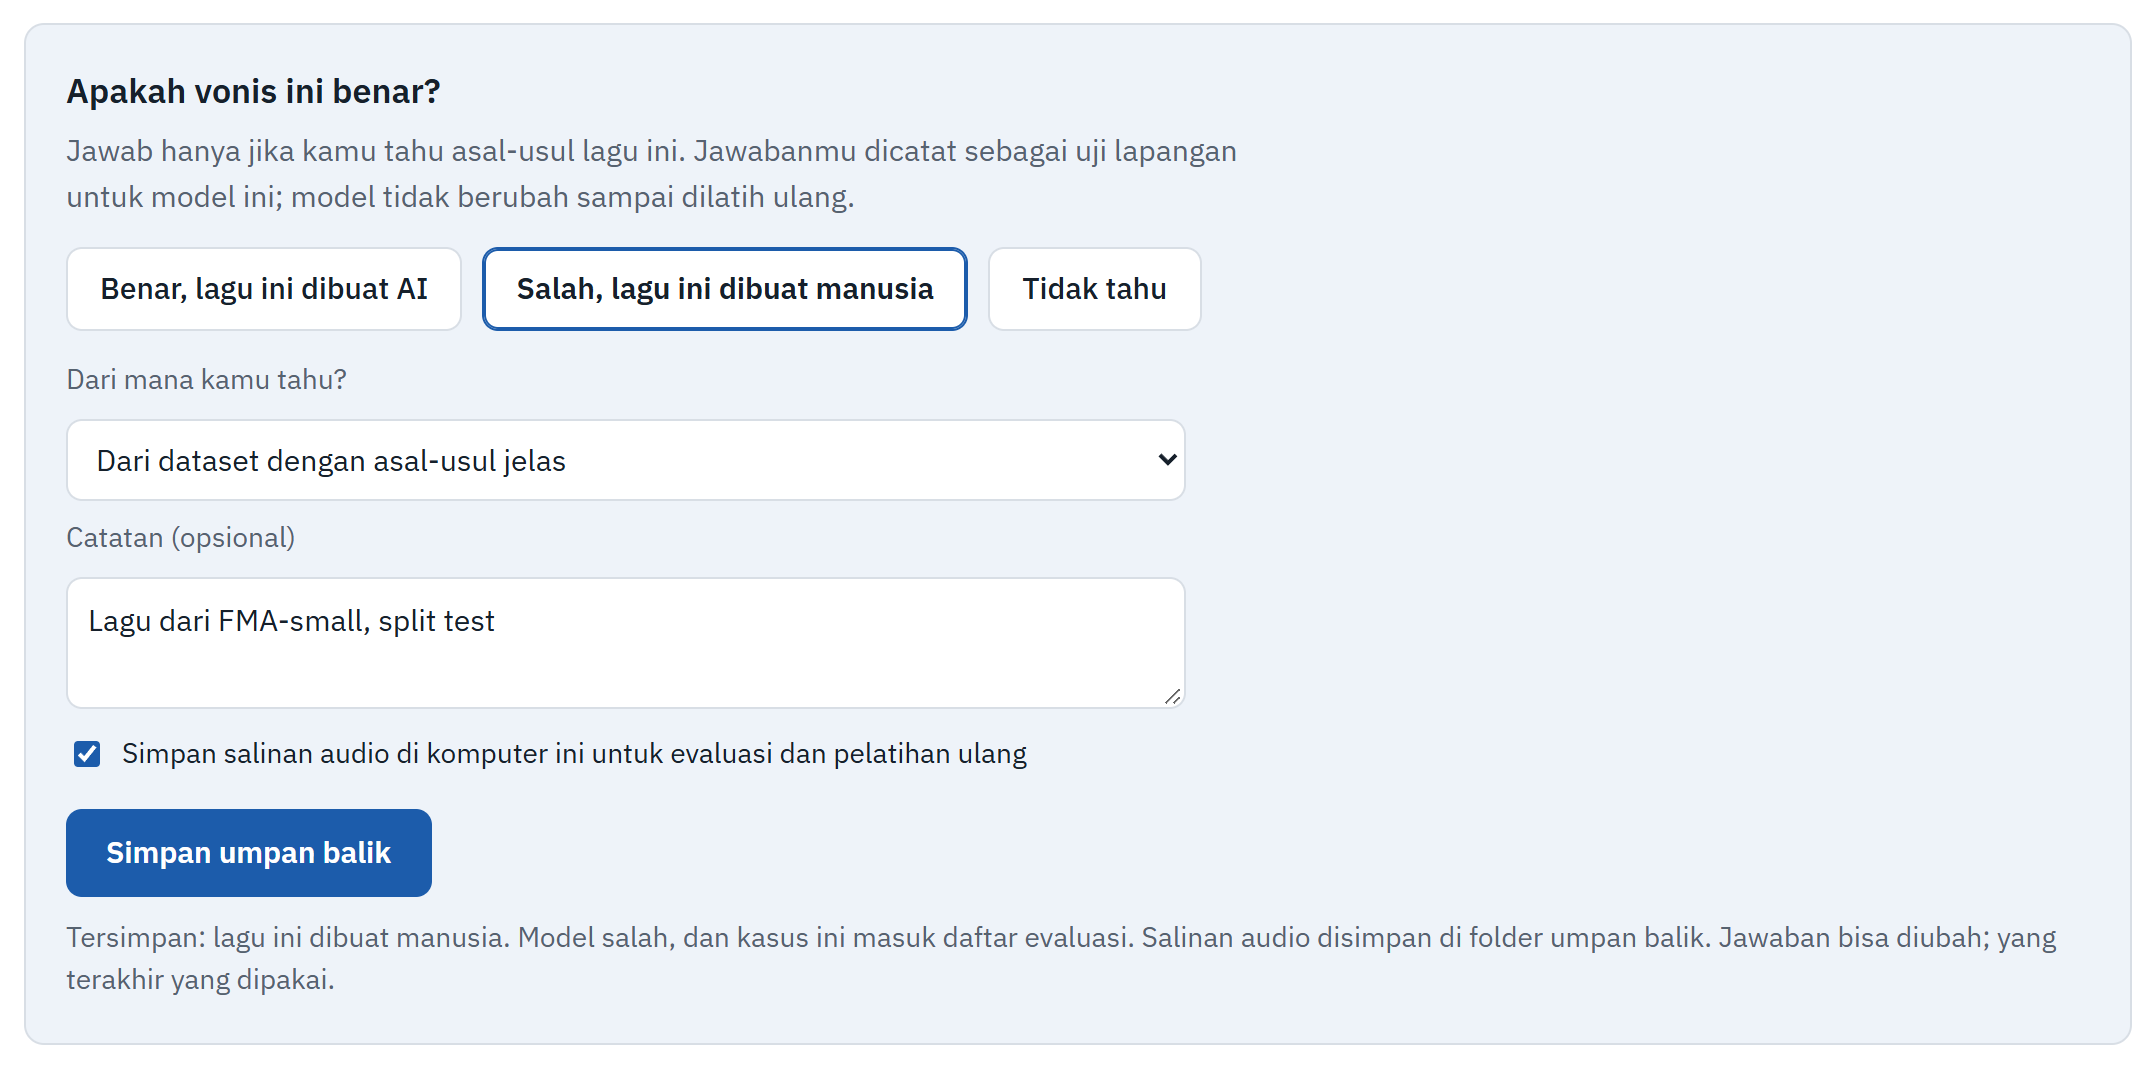
\includegraphics[width=0.9\textwidth]{11-umpan-balik-tersimpan.png}
\caption{Kartu umpan balik setelah disimpan.}
\label{fig:umpan-balik}
\end{figure}

Setiap jawaban disimpan sebagai satu baris di file \nolinkurl{data/feedback/feedback.jsonl}, berisi sidik jari file (SHA-256), nama file, nama run, vonis, skor, jawaban, label sebenarnya, sumber label, catatan, dan waktu. Panel \textbf{Uji lapangan} menampilkan akurasi beserta rentang 95\% Wilson, jumlah salah tuduh, jumlah lagu AI yang lolos, tabel benar dan salah, serta daftar kasus yang salah dinilai (Gambar~\ref{fig:uji-lapangan}).

\begin{figure}[htbp]
\centering
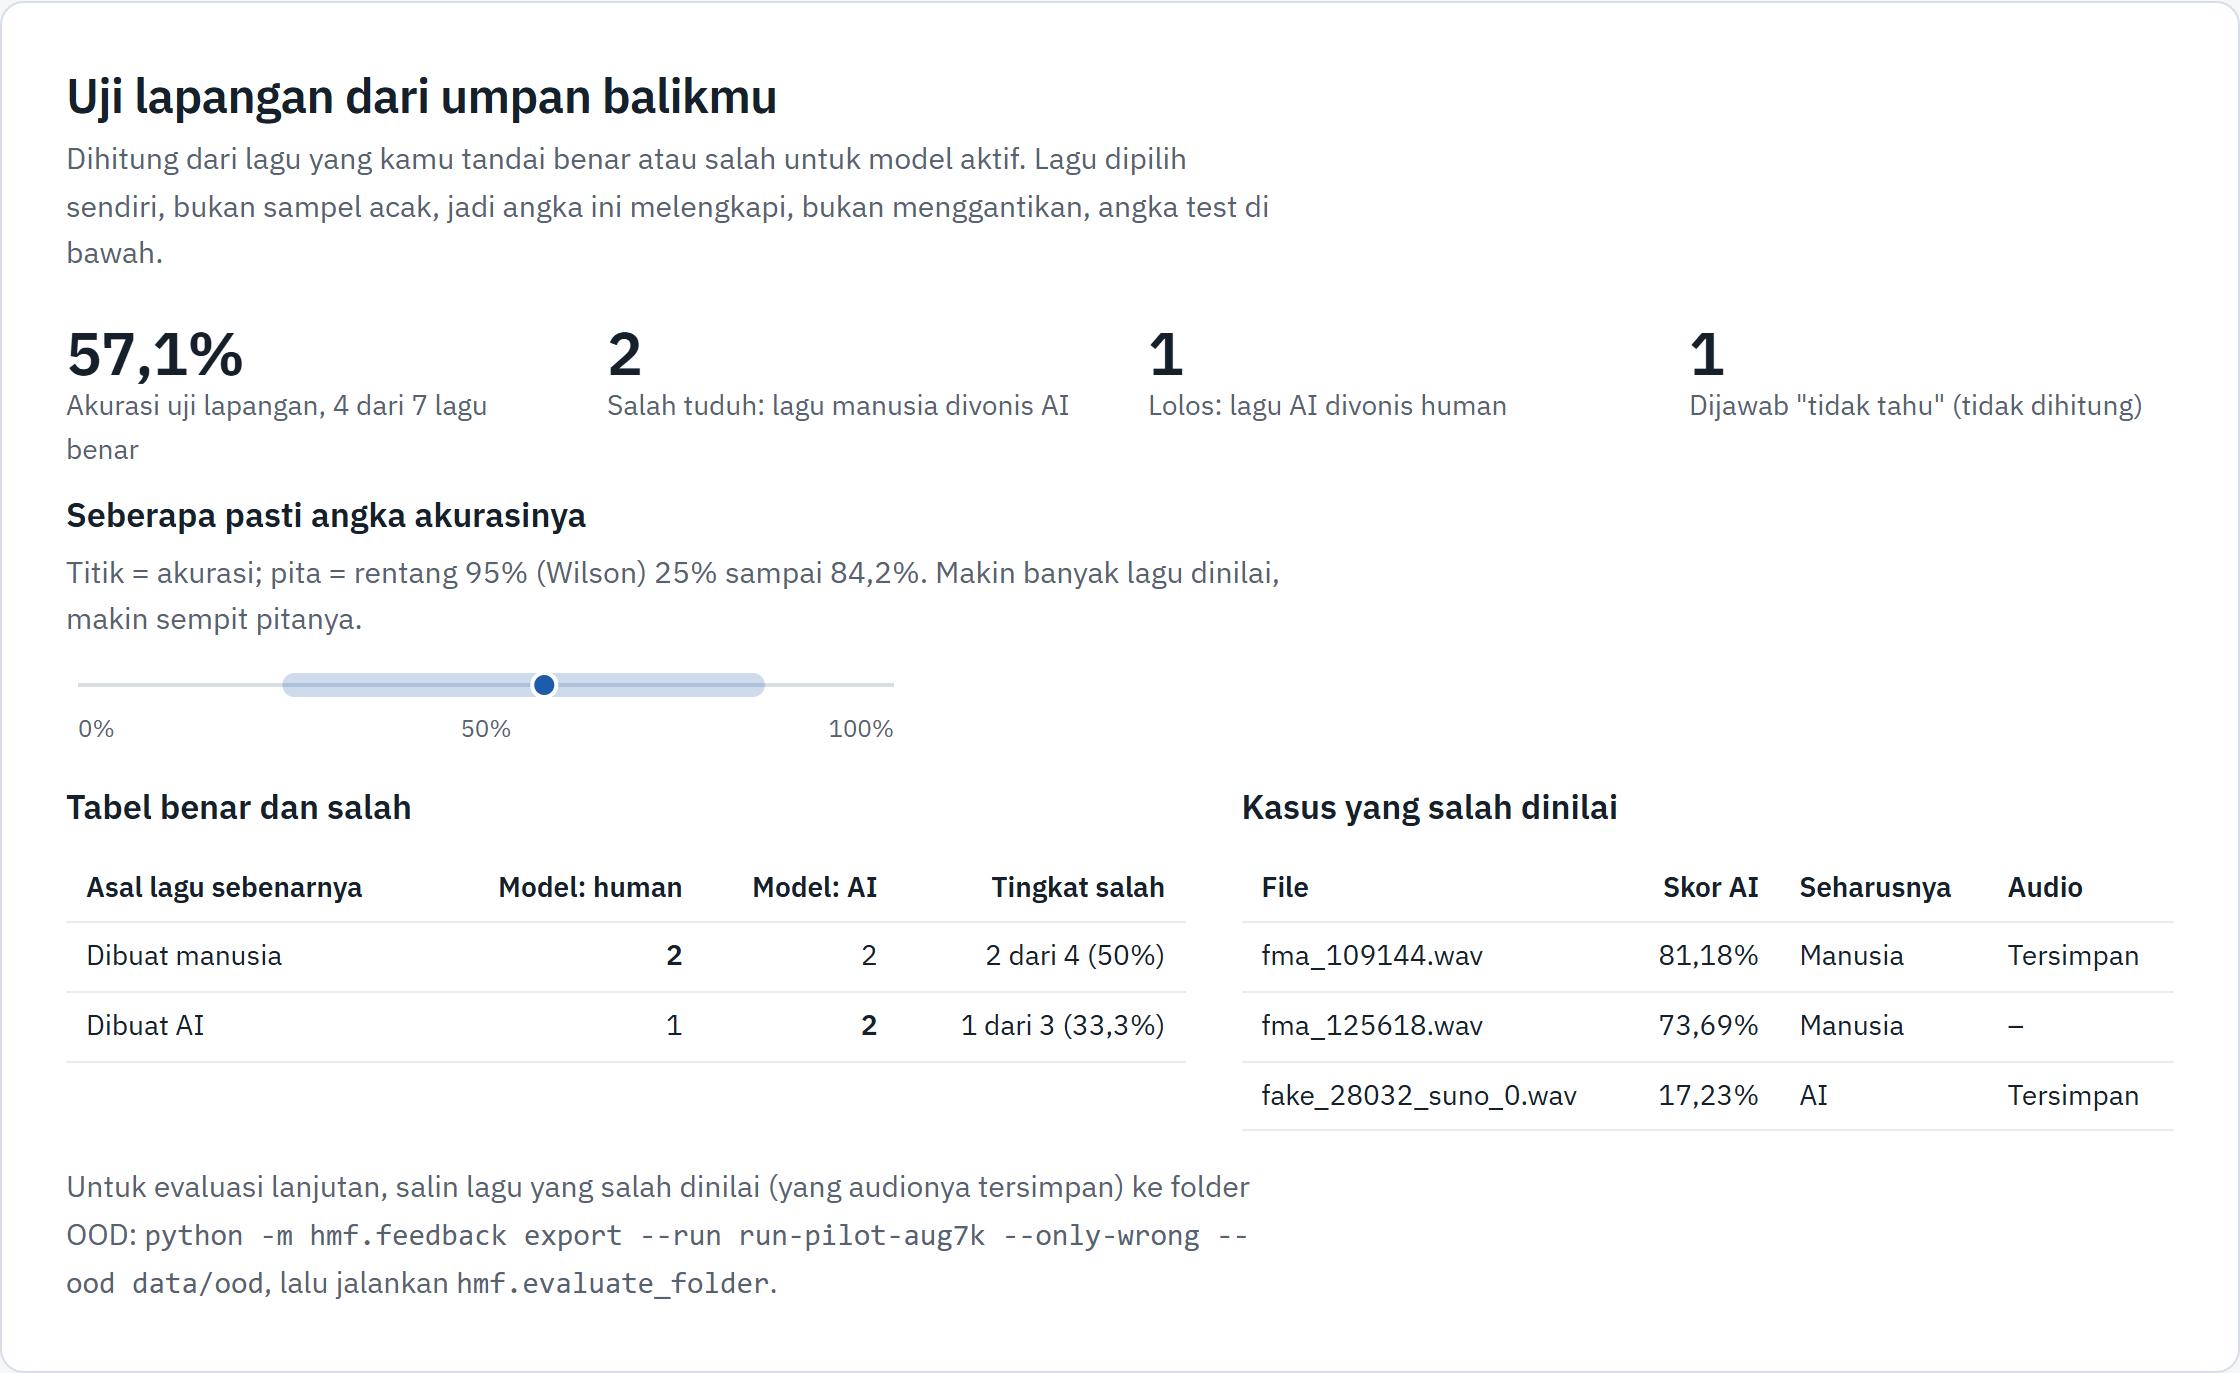
\includegraphics[width=0.95\textwidth]{12-uji-lapangan.png}
\caption{Panel uji lapangan: 4 dari 7 lagu benar dengan rentang 95\% 25--84\%.}
\label{fig:uji-lapangan}
\end{figure}

Lagu yang salah dinilai dapat dipakai untuk evaluasi lanjutan:
\begin{Perintah}
python -m hmf.feedback report --csv laporan.csv
python -m hmf.feedback export --run hmf-aug-v2 --only-wrong \
    --ood data/ood
python -m hmf.evaluate_folder --run runs/hmf-aug-v2 \
    --ai data/ood/ai --human data/ood/human
\end{Perintah}
Uji lapangan memiliki batasan: model tidak berubah sebelum dilatih ulang, lagu dipilih sendiri sehingga akurasinya tidak setara dengan angka test resmi, dan label berasal dari pengakuan pengguna. Lagu yang dipakai melatih ulang tidak boleh dipakai lagi untuk menguji model hasil pelatihan itu.

\section{Panel Tentang Model}
Panel di bagian bawah studio menunjukkan seberapa bisa dipercaya model yang aktif (Gambar~\ref{fig:panel-model}). Angkanya dibaca dari \kode{report.json} milik run tersebut dan diukur pada data test, bukan pada lagu yang diunggah. Panel memuat akurasi, \textit{balanced accuracy}, ROC AUC, jumlah lagu test, kurva loss train dan validasi per epoch, akurasi test per generator, serta konfigurasi audio. Akurasi per generator lebih berguna daripada akurasi total karena memperlihatkan generator yang sulit dideteksi.

\begin{figure}[htbp]
\centering
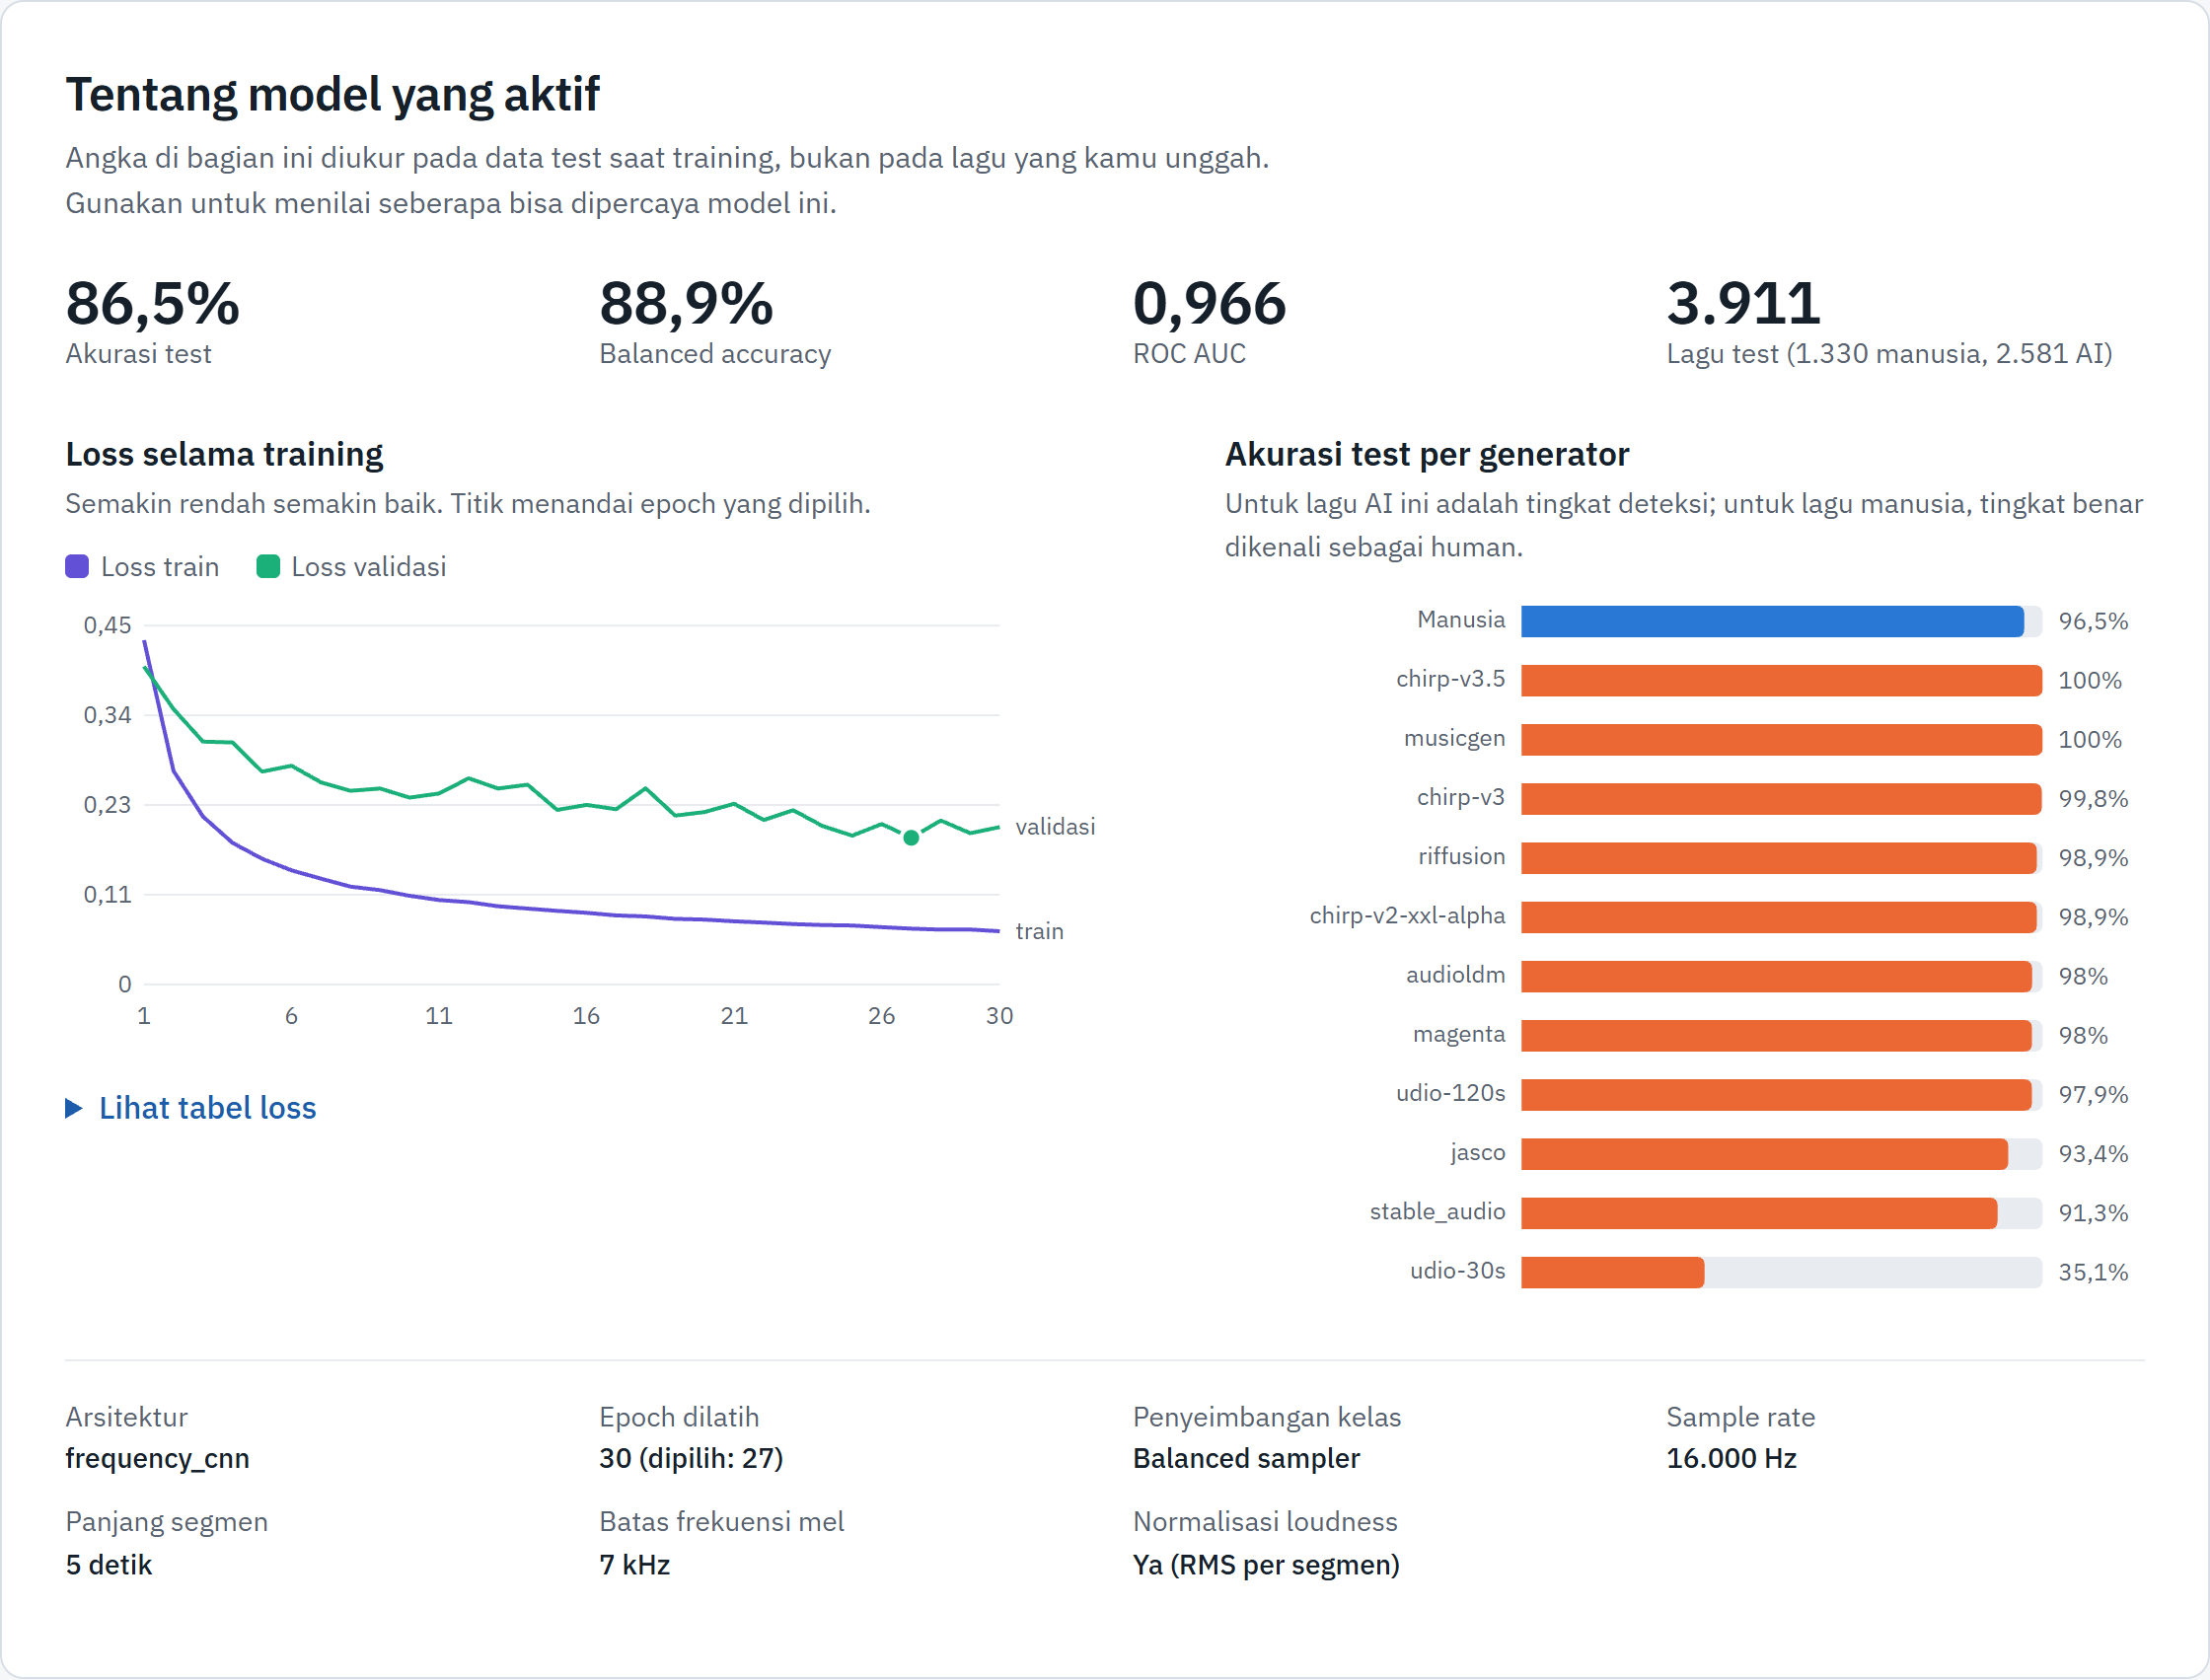
\includegraphics[width=0.95\textwidth]{06-tentang-model.png}
\caption{Panel Tentang model untuk model final \kode{hmf-aug-v2}.}
\label{fig:panel-model}
\end{figure}

\section{Melatih Ulang Model}
\begin{enumerate}
\item Unggah ke \kode{MyDrive/HMF/} di Google Drive: \kode{ai-music-detector-colab.zip} (kode dan manifest), \kode{fake\_songs.zip}, dan \kode{fma\_small.zip}.
\item Buka \kode{colab/train.ipynb} di Google Colab dan periksa sel konfigurasi (nama file, \kode{AUGMENT\_VARIANTS}, \kode{RUN\_NAME}).
\item \textbf{Sesi CPU:} jalankan semua sel dari atas. Notebook menyalin audio, mengunduh subset MUSEBENCH, membuat manifest, lalu menyiapkan fitur per 1.000 lagu. Setiap 100 lagu yang selesai disimpan ke Google Drive.
\item Jika sesi terputus, jalankan notebook lagi dari atas. Lagu yang sudah selesai tidak diproses ulang. Ulangi sampai muncul \kode{PREPARE SELESAI}.
\item \textbf{Sesi GPU:} ganti runtime ke GPU dan jalankan lagi dari atas. Pelatihan, uji \textit{robustness}, dan evaluasi OOD berjalan; pelatihan yang terhenti dilanjutkan otomatis dari epoch terakhir.
\item Salin folder \kode{MyDrive/HMF/runs/<RUN\_NAME>} ke folder \kode{runs/} di laptop, lalu buka dengan studio.
\end{enumerate}
Perintah inti tanpa notebook:
\begin{Perintah}
python -m hmf.manifest musebench --root <folder> \
    --reference-manifest data/manifest-28000.csv
python -m hmf.prepare --manifest <csv> --output <cache> \
    --augment-variants 3 --max-segments 6 --loudness-norm \
    --fmax 7000 --float16 --drop-duplicates \
    --resume --max-new-tracks 1000
python -m hmf.train --cache <cache> --output runs/<nama> \
    --epochs 30 --batch-size 64 --model frequency \
    --monitor loss --balance sampler \
    --balance-by generator --resume
\end{Perintah}
Cache fitur float16 berukuran $\pm$42 KB per segmen; dengan 3 varian dan 6 segmen per lagu, totalnya $\pm$20--25 GB untuk $\pm$36.000 lagu.

\section{Pemecahan Masalah}

{\singlespacing\small
\begin{longtable}{L{4.1cm} L{3.8cm} L{4.4cm}}
\caption{Pemecahan masalah umum.}\label{tab:masalah}\\
\toprule
Gejala & Penyebab & Solusi\\
\midrule
\endfirsthead
\toprule
Gejala & Penyebab & Solusi\\
\midrule
\endhead
\bottomrule
\endfoot
Port 8765 sudah dipakai & Studio lain masih berjalan & Hentikan studio lama dengan Ctrl+C atau pakai \kode{--port 8800}\\
Tidak ada run lengkap & Folder \kode{runs/} kosong atau run belum selesai & Salin folder run ke \kode{runs/} atau pilih dengan \kode{--run}\\
Audio gagal dibaca & Format tidak didukung atau file rusak & Konversi ke MP3 atau WAV, lalu coba lagi\\
File lebih dari 32 MB & Batas unggah studio & Potong rekaman atau kompres ke MP3\\
Pemutar audio tidak muncul & Browser tidak dapat memutar format itu & Analisis tetap dapat dijalankan\\
Skor berbeda dari sebelumnya & Model aktif berbeda & Periksa nama run di pojok kanan atas\\
Tidak dapat terhubung ke GPU di Colab & Kuota GPU gratis habis & Siapkan fitur di runtime CPU; lanjutkan pelatihan saat kuota kembali\\
Disk penuh saat menulis cache & Disk Colab tidak cukup & Kurangi \kode{AUGMENT\_VARIANTS} atau jumlah lagu MUSEBENCH sebelum sesi pertama\\
Duplicate audio bytes & File yang sama muncul dua kali & Tambahkan \kode{--drop-duplicates}\\
Pengaturan berbeda dari plan & Pengaturan diubah di tengah cicilan & Kembalikan pengaturan atau pakai \kode{RUN\_NAME} baru\\
\end{longtable}}

\chapter{HASIL DAN PEMBAHASAN}

\section{Data dan Pelatihan Model Final}
Model final (\kode{hmf-aug-v2}) dilatih dengan 35.766 lagu (Tabel~\ref{tab:data-final}). Pelatihan berjalan 30 epoch di GPU Google Colab dan dilanjutkan dari epoch 8 setelah sesi terputus. Epoch 27 dipilih karena loss validasinya terendah, yaitu 0,184 (Gambar~\ref{fig:loss}).

\begin{table}[htbp]
\centering
\singlespacing\small
\caption{Pembagian data model final.}
\label{tab:data-final}
\begin{tabular}{lrrrr}
\toprule
Bagian & Lagu & Manusia & AI & Segmen 5 detik\\
\midrule
Train & 28.587 (79,9\%) & 8.198 & 20.389 & 508.188\textsuperscript{a}\\
Validation & 3.268 (9,1\%) & 2.158 & 1.110 & 19.237\\
Test & 3.911 (10,9\%) & 1.330 & 2.581 & 23.083\\
\midrule
Total & 35.766 & 11.686 & 24.080 & \\
\bottomrule
\multicolumn{5}{l}{\footnotesize \textsuperscript{a} Termasuk 3 versi augmentasi codec per lagu.}
\end{tabular}
\end{table}

\begin{figure}[htbp]
\centering
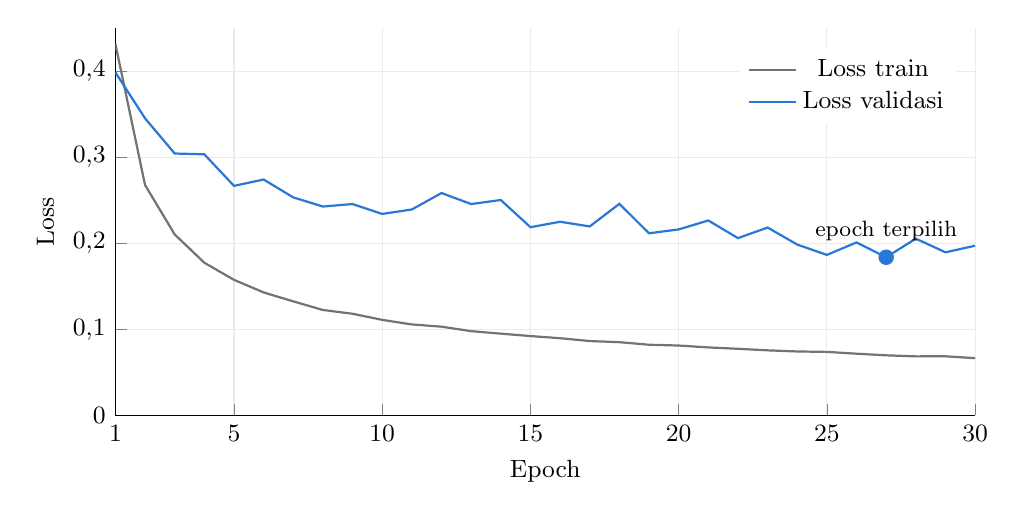
\begin{tikzpicture}
\begin{axis}[
  width=12.5cm, height=6.5cm,
  xmin=1, xmax=30, ymin=0, ymax=0.45,
  xtick={1,5,10,15,20,25,30},
  ytick={0,0.1,0.2,0.3,0.4},
  yticklabel style={/pgf/number format/.cd, use comma, fixed, precision=1},
  xlabel={Epoch}, ylabel={Loss},
  axis lines*=left, grid=major, grid style={black!8},
  legend style={draw=none, font=\small, at={(0.98,0.95)}, anchor=north east},
  tick label style={font=\small}, label style={font=\small}]
\addplot[thick, color=black!55] coordinates {(1,0.4317) (2,0.2678) (3,0.2104) (4,0.1775) (5,0.1576) (6,0.1430) (7,0.1326) (8,0.1226) (9,0.1182) (10,0.1111) (11,0.1058) (12,0.1032) (13,0.0980) (14,0.0951) (15,0.0923) (16,0.0898) (17,0.0865) (18,0.0852) (19,0.0822) (20,0.0813) (21,0.0791) (22,0.0775) (23,0.0757) (24,0.0744) (25,0.0739) (26,0.0718) (27,0.0699) (28,0.0687) (29,0.0688) (30,0.0666)};
\addlegendentry{Loss train}
\addplot[thick, color=aksen] coordinates {(1,0.3987) (2,0.3453) (3,0.3044) (4,0.3035) (5,0.2668) (6,0.2742) (7,0.2534) (8,0.2428) (9,0.2457) (10,0.2342) (11,0.2394) (12,0.2585) (13,0.2457) (14,0.2504) (15,0.2188) (16,0.2251) (17,0.2197) (18,0.2459) (19,0.2117) (20,0.2162) (21,0.2266) (22,0.2061) (23,0.2184) (24,0.1986) (25,0.1866) (26,0.2011) (27,0.1839) (28,0.2055) (29,0.1896) (30,0.1973)};
\addlegendentry{Loss validasi}
\addplot[only marks, mark=*, mark size=2.6pt, color=aksen, forget plot] coordinates {(27,0.1839)};
\node[font=\footnotesize, anchor=south] at (axis cs:27,0.192) {epoch terpilih};
\end{axis}
\end{tikzpicture}
\caption{Loss train dan validasi per epoch model final; titik menandai epoch 27 yang dipilih.}
\label{fig:loss}
\end{figure}

\section{Hasil Hold-Out Test}
Pada 3.911 lagu test, model final mencapai akurasi 86,5\% dan ROC AUC 0,966 (Tabel~\ref{tab:test}). Salah tuduh jarang terjadi: hanya 47 dari 1.330 lagu manusia (3,5\%) divonis AI (Tabel~\ref{tab:confusion}). Hampir semua kesalahan adalah lagu AI yang lolos sebagai manusia.

\begin{table}[htbp]
\centering
\singlespacing\small
\caption{Hasil hold-out test model final.}
\label{tab:test}
\begin{tabular}{lr}
\toprule
Metrik & Nilai\\
\midrule
Accuracy & 86,5\%\\
Balanced accuracy & 88,9\%\\
Macro F1 & 0,859\\
ROC AUC & 0,966\\
Recall manusia (lagu manusia benar dikenali) & 96,5\% (1.283 dari 1.330)\\
Recall AI (lagu AI terdeteksi) & 81,4\% (2.101 dari 2.581)\\
Presisi AI (vonis AI yang memang AI) & 97,8\%\\
\bottomrule
\end{tabular}
\end{table}

\begin{table}[htbp]
\centering
\singlespacing\small
\caption{Confusion matrix model final pada data test.}
\label{tab:confusion}
\begin{tabular}{lrr}
\toprule
Asal lagu sebenarnya & Divonis human & Divonis AI\\
\midrule
Manusia & 1.283 & 47\\
AI & 480 & 2.101\\
\bottomrule
\end{tabular}
\end{table}

\section{Recall per Generator}
Semua generator terdeteksi minimal 91\%, kecuali udio-30s yang hanya 35,1\% (Gambar~\ref{fig:per-generator}). Tanpa udio-30s, recall AI naik menjadi 98,5\% (1.857 dari 1.886 lagu). Generator udio-30s, chirp-v3, dan chirp-v2-xxl-alpha sama sekali tidak ada di data train dan hanya muncul di validation dan test. Dua versi Suno itu tetap terdeteksi sekitar 99\%, tetapi udio-30s tidak. Artinya, model dapat mengenali versi baru dari generator yang sudah dikenalnya, tetapi tidak selalu. Inilah batasan generalisasi yang paling penting.

\begin{figure}[htbp]
\centering
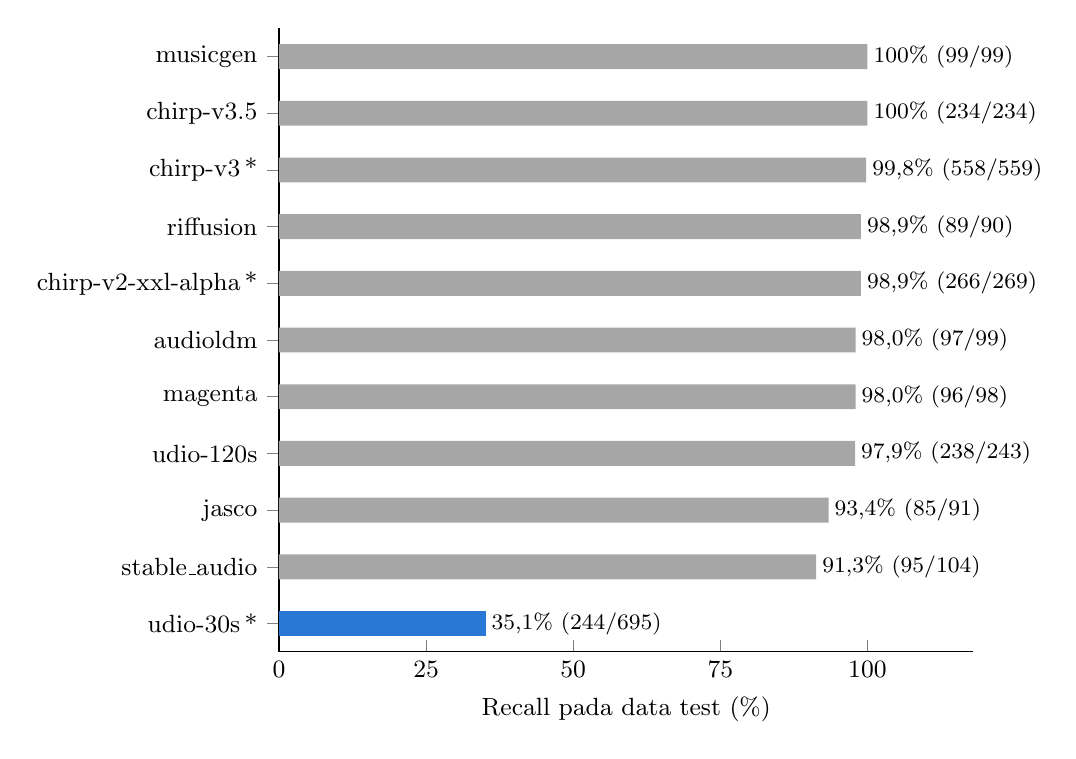
\begin{tikzpicture}
\begin{axis}[
  xbar, bar width=9pt, bar shift=0pt, y=0.72cm,
  xmin=0, xmax=118, xtick={0,25,50,75,100},
  ytick={1,...,11},
  yticklabels={udio-30s\,*, stable\_audio, jasco, udio-120s, magenta, audioldm, chirp-v2-xxl-alpha\,*, riffusion, chirp-v3\,*, chirp-v3.5, musicgen},
  xlabel={Recall pada data test (\%)},
  axis x line*=bottom, axis y line*=left,
  enlarge y limits=0.05, width=10.4cm,
  tick label style={font=\small}, label style={font=\small},
  clip=false]
\addplot[fill=black!35, draw=none] coordinates {
  (91.3,2) (93.4,3) (97.9,4) (98.0,5) (98.0,6) (98.9,7) (98.9,8) (99.8,9) (100,10) (100,11)};
\addplot[fill=aksen, draw=none] coordinates {(35.1,1)};
\foreach \x/\y/\t in {35.1/1/{35,1\% (244/695)}, 91.3/2/{91,3\% (95/104)}, 93.4/3/{93,4\% (85/91)},
  97.9/4/{97,9\% (238/243)}, 98.0/5/{98,0\% (96/98)}, 98.0/6/{98,0\% (97/99)},
  98.9/7/{98,9\% (266/269)}, 98.9/8/{98,9\% (89/90)}, 99.8/9/{99,8\% (558/559)},
  100/10/{100\% (234/234)}, 100/11/{100\% (99/99)}}
  {\edef\temp{\noexpand\node[anchor=west, font=\noexpand\footnotesize, inner sep=2pt] at (axis cs:\x,\y) {\unexpanded\expandafter{\t}};}\temp}
\end{axis}
\end{tikzpicture}
\caption{Recall per generator pada data test model final; tanda * berarti generator tidak ada di data train.}
\label{fig:per-generator}
\end{figure}

\section{Uji Robustness terhadap Kompresi Ulang}
Uji \textit{robustness} memakai 200 lagu test (100 per kelas) yang dikompres ulang dengan empat format, lalu membandingkan vonis model final sebelum dan sesudah kompresi (Tabel~\ref{tab:robust}).

\begin{table}[htbp]
\centering
\singlespacing\small
\caption{Hasil uji robustness model final.}
\label{tab:robust}
\begin{tabular}{lccc}
\toprule
Kondisi & Akurasi & Flip rate & Mean $|\Delta|$ skor\\
\midrule
Asli (clean) & 88,5\% & -- & --\\
MP3 32 kbps mono 16 kHz & 86,5\% & 5,0\% & 0,055\\
MP3 128 kbps & 88,0\% & 0,5\% & 0,012\\
AAC 128 kbps & 88,0\% & 0,5\% & 0,016\\
Opus 64 kbps & 86,0\% & 3,5\% & 0,035\\
\bottomrule
\end{tabular}
\end{table}

Akurasi model final bertahan di 86--88\% pada semua kondisi, dengan ROC AUC 0,959 pada file asli. Kondisi terberat, MP3 32 kbps mono 16 kHz, hanya menurunkan akurasi 2 poin dan membalik 5\% vonis; rata-rata perubahan skor hanya 0,055. Pada MP3 dan AAC 128 kbps, skor hampir tidak bergeser. Artinya, vonis model ditentukan oleh isi musik, bukan oleh format atau kualitas file.

\section{Studi Ablasi}
Studi ablasi menambahkan perbaikan satu per satu untuk melihat peran masing-masing. Percobaan dilakukan dalam skala kecil, yaitu 1.000 lagu dengan 2 epoch di CPU dan 20 lagu test per kelas (Tabel~\ref{tab:ablasi}).

\begin{table}[htbp]
\centering
\singlespacing\small
\caption{Studi ablasi skala kecil.}
\label{tab:ablasi}
\begin{tabularx}{\textwidth}{Y L{2.5cm} L{1.4cm} L{2.0cm} L{1.6cm}}
\toprule
Model & Skor manusia: asli $\rightarrow$ MP3 32k & Flip MP3 32k & $|\Delta|$ kondisi terburuk & Akurasi asli\\
\midrule
Tanpa augmentasi & 0,00 $\rightarrow$ 1,00 & 50\% & 0,501 & 100\%\\
Augmentasi tanpa \kode{--fmax} & 0,04 $\rightarrow$ 0,91 & 50\% & 0,442 & 100\%\\
Augmentasi dan \kode{--fmax 7000} & 0,33 $\rightarrow$ 0,33 & 0\% & 0,008 & 77,5\%\\
\bottomrule
\end{tabularx}
\end{table}

Augmentasi saja belum cukup: vonis tetap berbalik pada 50\% lagu. Baru setelah spektrogram dibatasi sampai 7 kHz, skor tidak lagi berubah oleh codec. Akurasi 100\% pada dua baris pertama berasal dari petunjuk kualitas file, sehingga langsung runtuh begitu lagu manusia dikompres. Angka akurasi pada tabel ini berasal dari model kecil 2 epoch; yang dibaca adalah polanya.

\section{Hasil Pengujian Perangkat Lunak}\label{sec:hasil-blackbox}
Seluruh 42 tes otomatis pytest lulus. Hasil \textit{black-box testing} studio web disajikan pada Tabel~\ref{tab:blackbox}. Skenario ini menguji perilaku aplikasi, bukan akurasi model.

{\singlespacing\small
\begin{longtable}{L{0.5cm} L{2.3cm} L{3.2cm} L{4.4cm} L{1.2cm}}
\caption{Hasil black-box testing studio web.}\label{tab:blackbox}\\
\toprule
No & Skenario & Masukan & Hasil yang diharapkan & Hasil\\
\midrule
\endfirsthead
\toprule
No & Skenario & Masukan & Hasil yang diharapkan & Hasil\\
\midrule
\endhead
\bottomrule
\endfoot
1 & Membuka studio & Buka \url{http://127.0.0.1:8765} & Halaman tampil dengan nama model aktif & Sesuai\\
2 & Analisis lagu & MP3 2 menit & Vonis, skor AI, spektrogram, dan 24 batang skor segmen tampil & Sesuai\\
3 & Kecocokan skor & Lagu yang sama & Persentase di layar sama dengan \kode{ai\_score} di JSON & Sesuai\\
4 & File bukan audio & File teks & Pesan ``Audio gagal dibaca'' & Sesuai\\
5 & Port sudah dipakai & Studio kedua di port yang sama & Server menolak berjalan dan menyarankan port lain & Sesuai\\
6 & Simpan umpan balik & Tandai vonis salah, pilih sumber label, simpan audio & Umpan balik tersimpan; panel uji lapangan bertambah & Sesuai\\
7 & Audio berbeda & File lain dikirim sebagai audio umpan balik & Ditolak dengan pesan ``File berbeda dari lagu yang dianalisis'' & Sesuai\\
8 & Tampilan ponsel & Lebar layar 375 piksel & Semua bagian tersusun satu kolom tanpa geser ke samping & Sesuai\\
\end{longtable}}

\section{Pembahasan dan Keterbatasan}
Hasil di atas menjawab rumusan masalah. Detektor tidak bergantung pada format file: vonisnya stabil pada empat kondisi kompresi ulang. Akurasi test 86,5\% dengan ROC AUC 0,966 mencerminkan kemampuan yang sebenarnya karena data latih sudah diaugmentasi dan dibatasi sampai 7 kHz, sehingga petunjuk codec tidak bisa dipakai. Model juga berhati-hati: hanya 3,5\% lagu manusia yang salah dituduh AI. Hasil deteksi disajikan secara transparan melalui skor per segmen, spektrogram, dan panel model.

Keterbatasan yang perlu diperhatikan:
\begin{itemize}
\item Model hanya mengenali pola yang ada di data latih. Generator yang belum pernah dilihat, seperti udio-30s, dapat lolos sebagai manusia.
\item Ambang 0,5 belum dikalibrasi; skor 51\% tidak berarti peluang 51\% bahwa lagu itu buatan AI.
\item Spektrogram hanya sampai 7 kHz, sehingga artefak AI di frekuensi tinggi tidak terlihat oleh model.
\item Lagu campuran manusia dan AI belum menjadi kelas tersendiri.
\item Sebagian besar kesalahan adalah lagu AI yang lolos sebagai manusia (480 dari 2.581 lagu AI), terutama dari udio-30s.
\end{itemize}

Hasil studio tidak boleh dipakai sebagai satu-satunya dasar untuk menuduh seseorang memakai AI. Skor sebaiknya dilaporkan sebagai perkiraan bersama nama model dan grafik per segmen, serta digabungkan dengan bukti lain seperti file proyek atau rekaman sesi.

\chapter{PENUTUP}

\section{Kesimpulan}
\begin{enumerate}
\item Aplikasi \textit{AI Music Detector} berhasil dibangun sebagai studio web lokal yang menganalisis rekaman musik tanpa mengirim audio ke layanan luar. Setiap vonis disertai skor per segmen 5 detik dan spektrogram yang dilihat model.
\item \textit{Shortcut learning} terhadap codec dicegah dengan augmentasi codec untuk kedua kelas, normalisasi loudness, dan pembatasan spektrogram sampai 7 kHz. Studi ablasi menunjukkan pembatasan 7 kHz adalah komponen kunci: tanpanya, vonis masih berbalik pada separuh lagu yang dikompres ulang.
\item Model final mencapai akurasi 86,5\%, \textit{balanced accuracy} 88,9\%, dan ROC AUC 0,966 pada 3.911 lagu test, dengan salah tuduh hanya 3,5\%. Pada kompresi ulang, akurasinya bertahan di 86--88\% dan hanya 5\% vonis yang berbalik.
\item Kelemahan utama ada pada generator yang tidak ada di data latih: udio-30s hanya terdeteksi 35,1\%, meskipun dua versi Suno yang juga tidak dilatih tetap terdeteksi sekitar 99\%.
\end{enumerate}

\section{Saran}
\begin{enumerate}
\item Menambah contoh lagu dari generator terbaru, terutama Udio dan Suno versi baru, lalu melatih ulang model memakai cache tambahan tanpa memproses ulang seluruh data.
\item Menjalankan evaluasi \textit{leave-one-generator-out} untuk setiap generator agar kemampuan generalisasi terukur lebih lengkap.
\item Mengumpulkan umpan balik pengguna pada lagu yang asal-usulnya jelas sebagai uji lapangan, dengan sebagian lagu disisihkan khusus untuk evaluasi.
\item Mengkalibrasi ambang keputusan dan mengulang \textit{black-box testing} memakai model final.
\end{enumerate}


\chapter*{DAFTAR PUSTAKA}
\addcontentsline{toc}{chapter}{DAFTAR PUSTAKA}
\begingroup
\singlespacing
\printbibliography[heading=none]
\endgroup

\chapter*{LAMPIRAN}
\addcontentsline{toc}{chapter}{LAMPIRAN}

\section*{Lampiran A. Struktur Folder Proyek}
\addcontentsline{toc}{section}{Lampiran A. Struktur Folder Proyek}
Kode sumber lengkap tersedia di \url{\RepoURL}.

{\singlespacing\small
\begin{longtable}{L{5.3cm} L{7.0cm}}
\toprule
Path & Isi\\
\midrule
\endfirsthead
\toprule
Path & Isi\\
\midrule
\endhead
\bottomrule
\endfoot
\kode{hmf/audio.py} & Dekode, augmentasi codec, normalisasi loudness, spektrogram log-Mel\\
\kode{hmf/prepare.py} & Membuat cache fitur dari manifest (augmentasi, cicilan, duplikat)\\
\kode{hmf/train.py} & Pelatihan CNN, \textit{balanced sampler}, metrik per generator, lanjutan pelatihan\\
\kode{hmf/model.py} & Arsitektur CNN\\
\kode{hmf/predict.py} & Analisis satu file dan ringkasan model\\
\kode{hmf/web.py},\newline \kode{hmf/studio.html} & Server dan halaman studio web\\
\kode{hmf/feedback.py} & Umpan balik pengguna: simpan, ringkas, dan ekspor\\
\kode{hmf/manifest.py} & Manifest MUSEBENCH dan \textit{leave-one-generator-out}\\
\kode{hmf/evaluate\_folder.py} & Evaluasi OOD dan uji \textit{robustness}\\
\kode{hmf/finalize.py} & Membuat \kode{report.json} untuk run yang terhenti\\
\kode{scripts/musebench\_index.py} & Memetakan dan mengunduh sebagian isi MUSEBENCH\\
\kode{colab/train.ipynb} & Notebook pelatihan di Google Colab\\
\kode{tests/} & Tes otomatis (pytest)\\
\kode{runs/hmf-aug-v2/} & Model final siap pakai: \kode{best.pt}, \kode{report.json}, \kode{history.json}, dan konfigurasi (Tabel~\ref{tab:file-model})\\
\kode{docs/manual/} & Buku manual ini beserta sumber LaTeX-nya\\
\end{longtable}}

\section*{Lampiran B. Daftar Perintah}
\addcontentsline{toc}{section}{Lampiran B. Daftar Perintah}
Di Windows, ganti \kode{python} dengan \kode{.\textbackslash.venv\textbackslash Scripts\textbackslash python.exe}.
\begin{Perintah}
# Jalankan tes otomatis
python -m pytest -q
# Studio web
python -m hmf.web --run runs/<nama> --port 8765
# Analisis satu file di terminal
python -m hmf.predict --run runs/<nama> --audio lagu.mp3
# Evaluasi OOD dan robustness
python -m hmf.evaluate_folder --run runs/<nama> \
    --ai <folder> --human <folder>
# Manifest MUSEBENCH dan leave-one-generator-out
python -m hmf.manifest musebench --root <folder>
python -m hmf.manifest logo --manifest <a.csv> <b.csv> \
    --holdout musicgen --output <logo.csv>
# Cache fitur dan pelatihan
python -m hmf.prepare --manifest <csv> --output <cache> ...
python -m hmf.train --cache <cache> --output runs/<nama> ...
# Lanjutkan pelatihan yang terhenti / report.json sementara
python -m hmf.train --cache <cache> --output runs/<nama> --resume ...
python -m hmf.finalize --cache <cache> --run runs/<nama>
# Umpan balik pengguna
python -m hmf.feedback report --csv laporan.csv
python -m hmf.feedback export --run <nama> --only-wrong --ood data/ood
\end{Perintah}

\section*{Lampiran C. Contoh Laporan JSON}
\addcontentsline{toc}{section}{Lampiran C. Contoh Laporan JSON}
Keluaran model final pada berkas demo sintetis 8 detik dari repositori, dihasilkan dengan perintah berikut. Laporan yang diunduh dari studio juga memuat daftar \kode{segment\_scores}.
\begin{Perintah}
python -m hmf.predict --run runs/hmf-aug-v2 \
    --audio data/demo/test_1_0.wav
\end{Perintah}
\begin{Perintah}
{
  "status": "completed",
  "filename": "test_1_0.wav",
  "analysis_level": "track_classification",
  "result": {
    "verdict": "Human",
    "ai_score": 4.514792272083956e-05,
    "decision_threshold": 0.5,
    "aggregation": "mean_segment_score",
    "segment_seconds": 5.0,
    "segments_analyzed": 2
  },
  "metadata": {
    "model": "frequency_cnn",
    "models_used": 1,
    "run": "hmf-aug-v2",
    "processing_time_seconds": 20.916
  }
}
\end{Perintah}

\section*{Lampiran D. Sumber Data, Tautan, dan Lisensi}
\addcontentsline{toc}{section}{Lampiran D. Sumber Data, Tautan, dan Lisensi}
Dataset yang dipakai melatih model final:
\begin{itemize}
\item SONICS: \url{https://arxiv.org/pdf/2408.14080} (makalah ICLR 2025: \url{https://iclr.cc/virtual/2025/poster/32089})
\item FMA (Free Music Archive): \url{https://github.com/mdeff/fma}
\item MUSEBENCH: \url{https://arxiv.org/abs/2610.20310}
\end{itemize}
Dataset dan penelitian terkait lainnya:
\begin{itemize}
\item FakeMusicCaps: \url{https://arxiv.org/html/2409.10684v2}
\item Improved robustness in AI-generated music detection (Suno v5): \url{https://arxiv.org/html/2607.27454}
\item The AI Music Arms Race (TISMIR): \url{https://transactions.ismir.net/articles/10.5334/tismir.254}
\item Echoes dataset: \url{https://arxiv.org/pdf/2603.23667}
\item Hard-negative robustness task: \url{https://arxiv.org/pdf/2608.14916}
\item Broadcast monitoring evaluation: \url{https://arxiv.org/pdf/2608.07359}
\item Stem-agnostic hybrid AI music detection: \url{https://arxiv.org/pdf/2609.26956}
\end{itemize}
Lisensi:
\begin{itemize}
\item MUSEBENCH: secara umum CC BY-SA 3.0; lagu Jamendo mengikuti lisensi per lagu; keluaran generator umumnya untuk keperluan nonkomersial.
\item SONICS dan FMA mengikuti lisensi masing-masing dataset.
\item Audio dataset tidak didistribusikan ulang bersama kode; repositori hanya berisi kode, manifest, dan dokumentasi.
\item Model dilatih dari bobot acak tanpa bobot pralatih.
\end{itemize}

\end{document}
